%=================AVANCES Y PRUEBAS=================
% SENSORES DE PULSO

\section{Sensor de pulso}
%Para determinar si los sensores de pulso elegidos funcionarían para el cálculo de la frecuencia cardíaca de un paciente, se realizaron pruebas unitarias con el fin de  visualizar la onda de salida entregada por ambos sensores en un osciloscopio y verificar su funcionamiento.\\

El procedimiento llevado a cabo con el sensor de pulso en este Trabajo Terminal, se realizó en las cuatro etapas descritas a continuación:

%Para determinar si el sensor de pulso elegido funcionaría para el cálculo de la frecuencia cardíaca de un paciente, se realizaron pruebas unitarias con el fin de visualizar la onda de salida en un osciloscopio y así verificar su funcionamiento. \\

\begin{itemize}
	\item \textbf{Prueba de funcionamiento:} En esta fase se conectó el sensor de acuerdo a lo especificado en su hoja de datos y la señal analógica obtenida se visualizó en el osciloscopio.
	\item \textbf{Digitalización de señal:} En esta fase se realizó el código en lenguaje ensamblador y C para digitalizar la señal con el uso del convertidor analógico-digital (ADC) del microcontrolador y se envió a una PC para la visualización de los valores resultantes de la conversión.
	\item \textbf{Procesamiento digital de señal:} El procesamiento digital de la señal consistió en la implementación del algoritmo de autocorrelación para el análisis del espectro de frecuencias y el cálculo de la frecuencia cardíaca.
	\item \textbf{Pruebas unitarias:} En esta fase se verificó que utilizando en el sensor y el algoritmo programado se obtuviera el resultado esperado de frecuencia cardíaca.
\end{itemize}

\subsection{Prueba de funcionamiento}
%\subsubsection{AD8232}
%El primer sensor que fue probado fue el AD8232, el cual es de tipo ECG y utiliza tres electrodos que se deben colocar en el brazo izquierdo y derecho, y la pierna derecha.\\
%
%Se realizó una prueba unitaria para comprobar el correcto funcionamiento del sensor, así como para verificar que la señal analógica entregada por el mismo sea de utilidad para calcular la frecuencia cardíaca del paciente. Para esta prueba el sensor fue alimentado con 3.3 V mediante las terminales 3.3v y GND,haciendo uso de un módulo FT232 como se muestra en la figura \ref{fig:AD8232Sensor}.\\


%\begin{figure}[htbp!]
%	\centering
%	\fbox{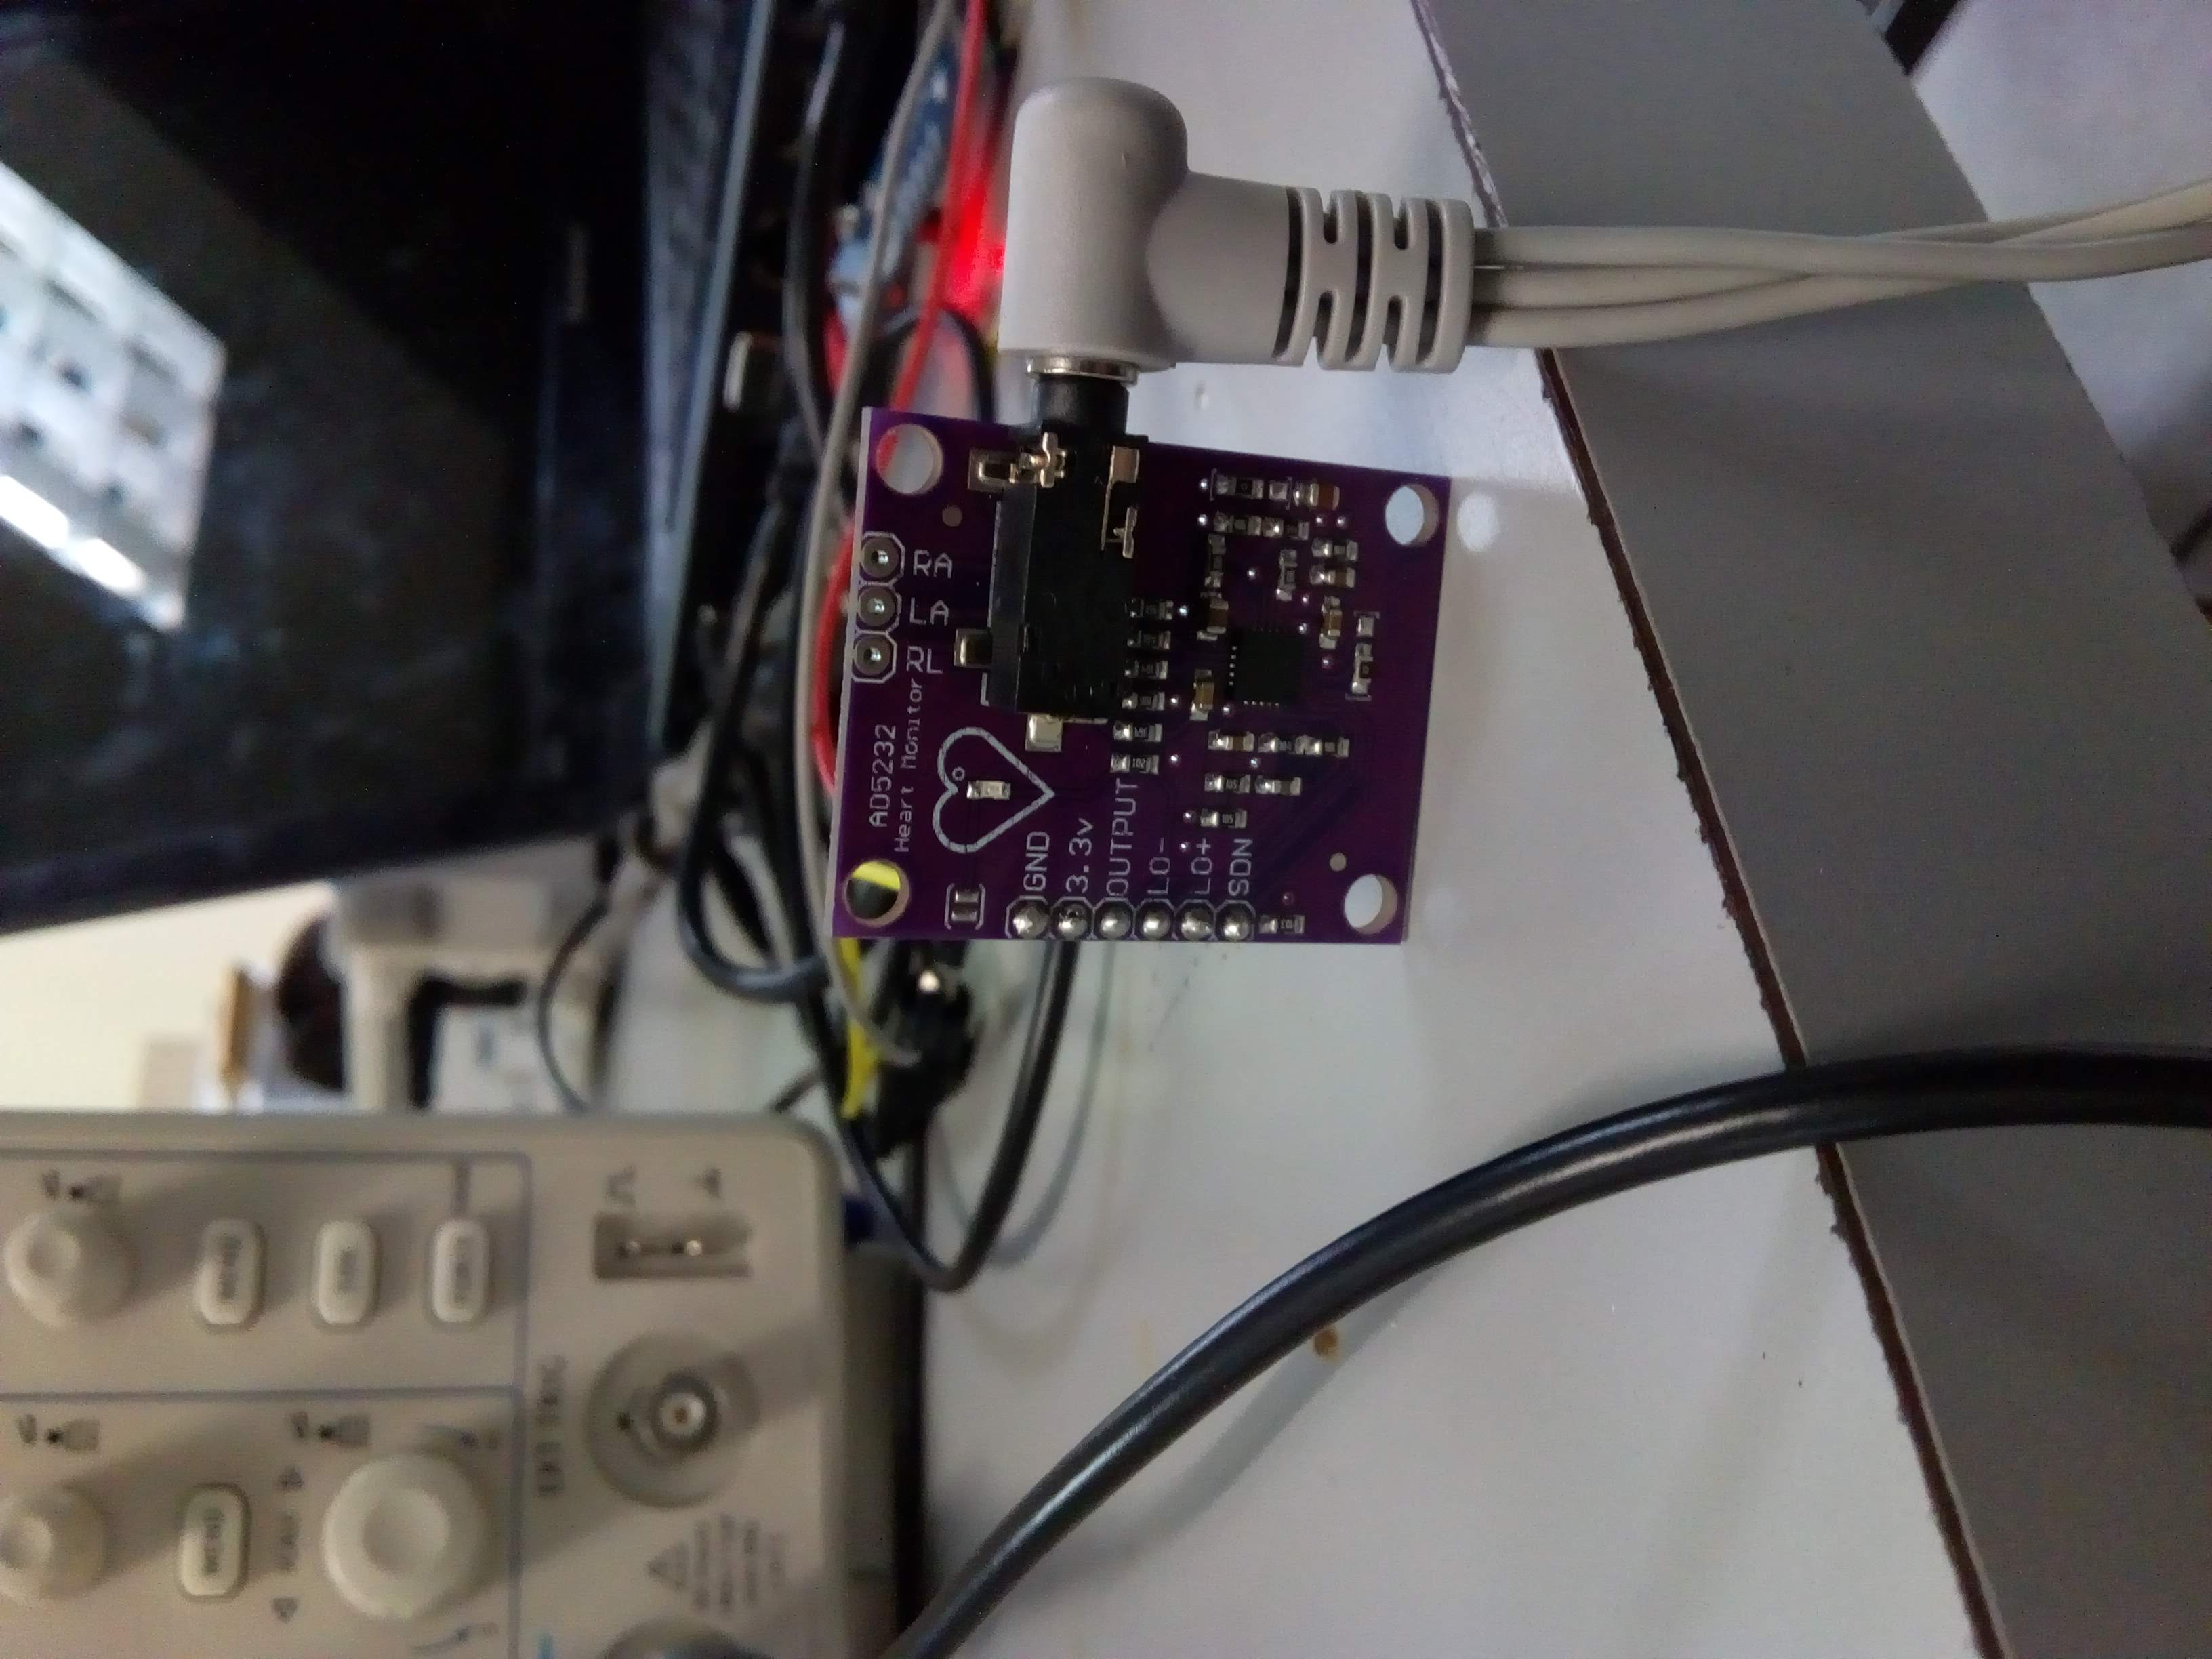
\includegraphics[width=0.6\textwidth]{AvancesPruebas/imagenes/AD8232-1.jpg}}
%	\caption{Sensor de pulso AD8232.}
%	\label{fig:AD8232Sensor}
%\end{figure}
%
%
%Una vez conectado correctamente, se colocaron los electrodos en el brazo derecho, brazo izquierdo y pierna derecha, respetando el color asignado a cada uno (verde, rojo y amarillo respectivamente) como se muestra en la figura \ref{fig:AD8232Electrodo}.\\
%\begin{figure}[htbp!]
%	\centering
%	\fbox{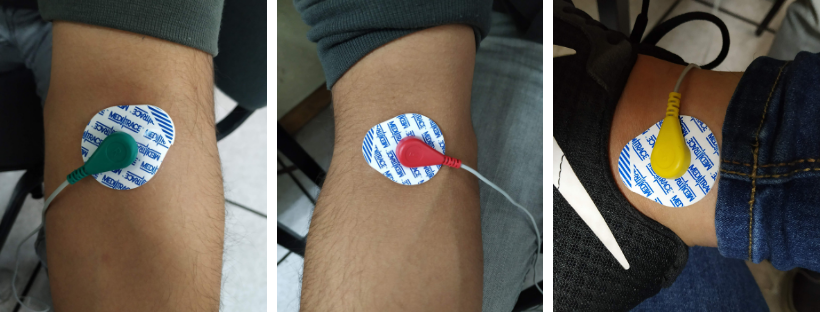
\includegraphics[width=1\textwidth]{AvancesPruebas/imagenes/AD8232-2.png}}
%	\caption{Electrodos conectados el sensor de pulso AD8232.}
%	\label{fig:AD8232Electrodo}
%\end{figure}
%
%La señal entregada por el sensor AD8232 se muestra en la figura \ref{fig:AD8232Osciloscopio}, a partir de esta señal podemos determinar que el sensor AD8232 proporciona una señal que puede ser útil para la detección de la frecuencia cardíaca, por lo que más adelante se realizarán pruebas con la señal digitalizada y procesada mediante un algoritmo.\\
%\begin{figure}[htbp!]
%	\centering
%	\fbox{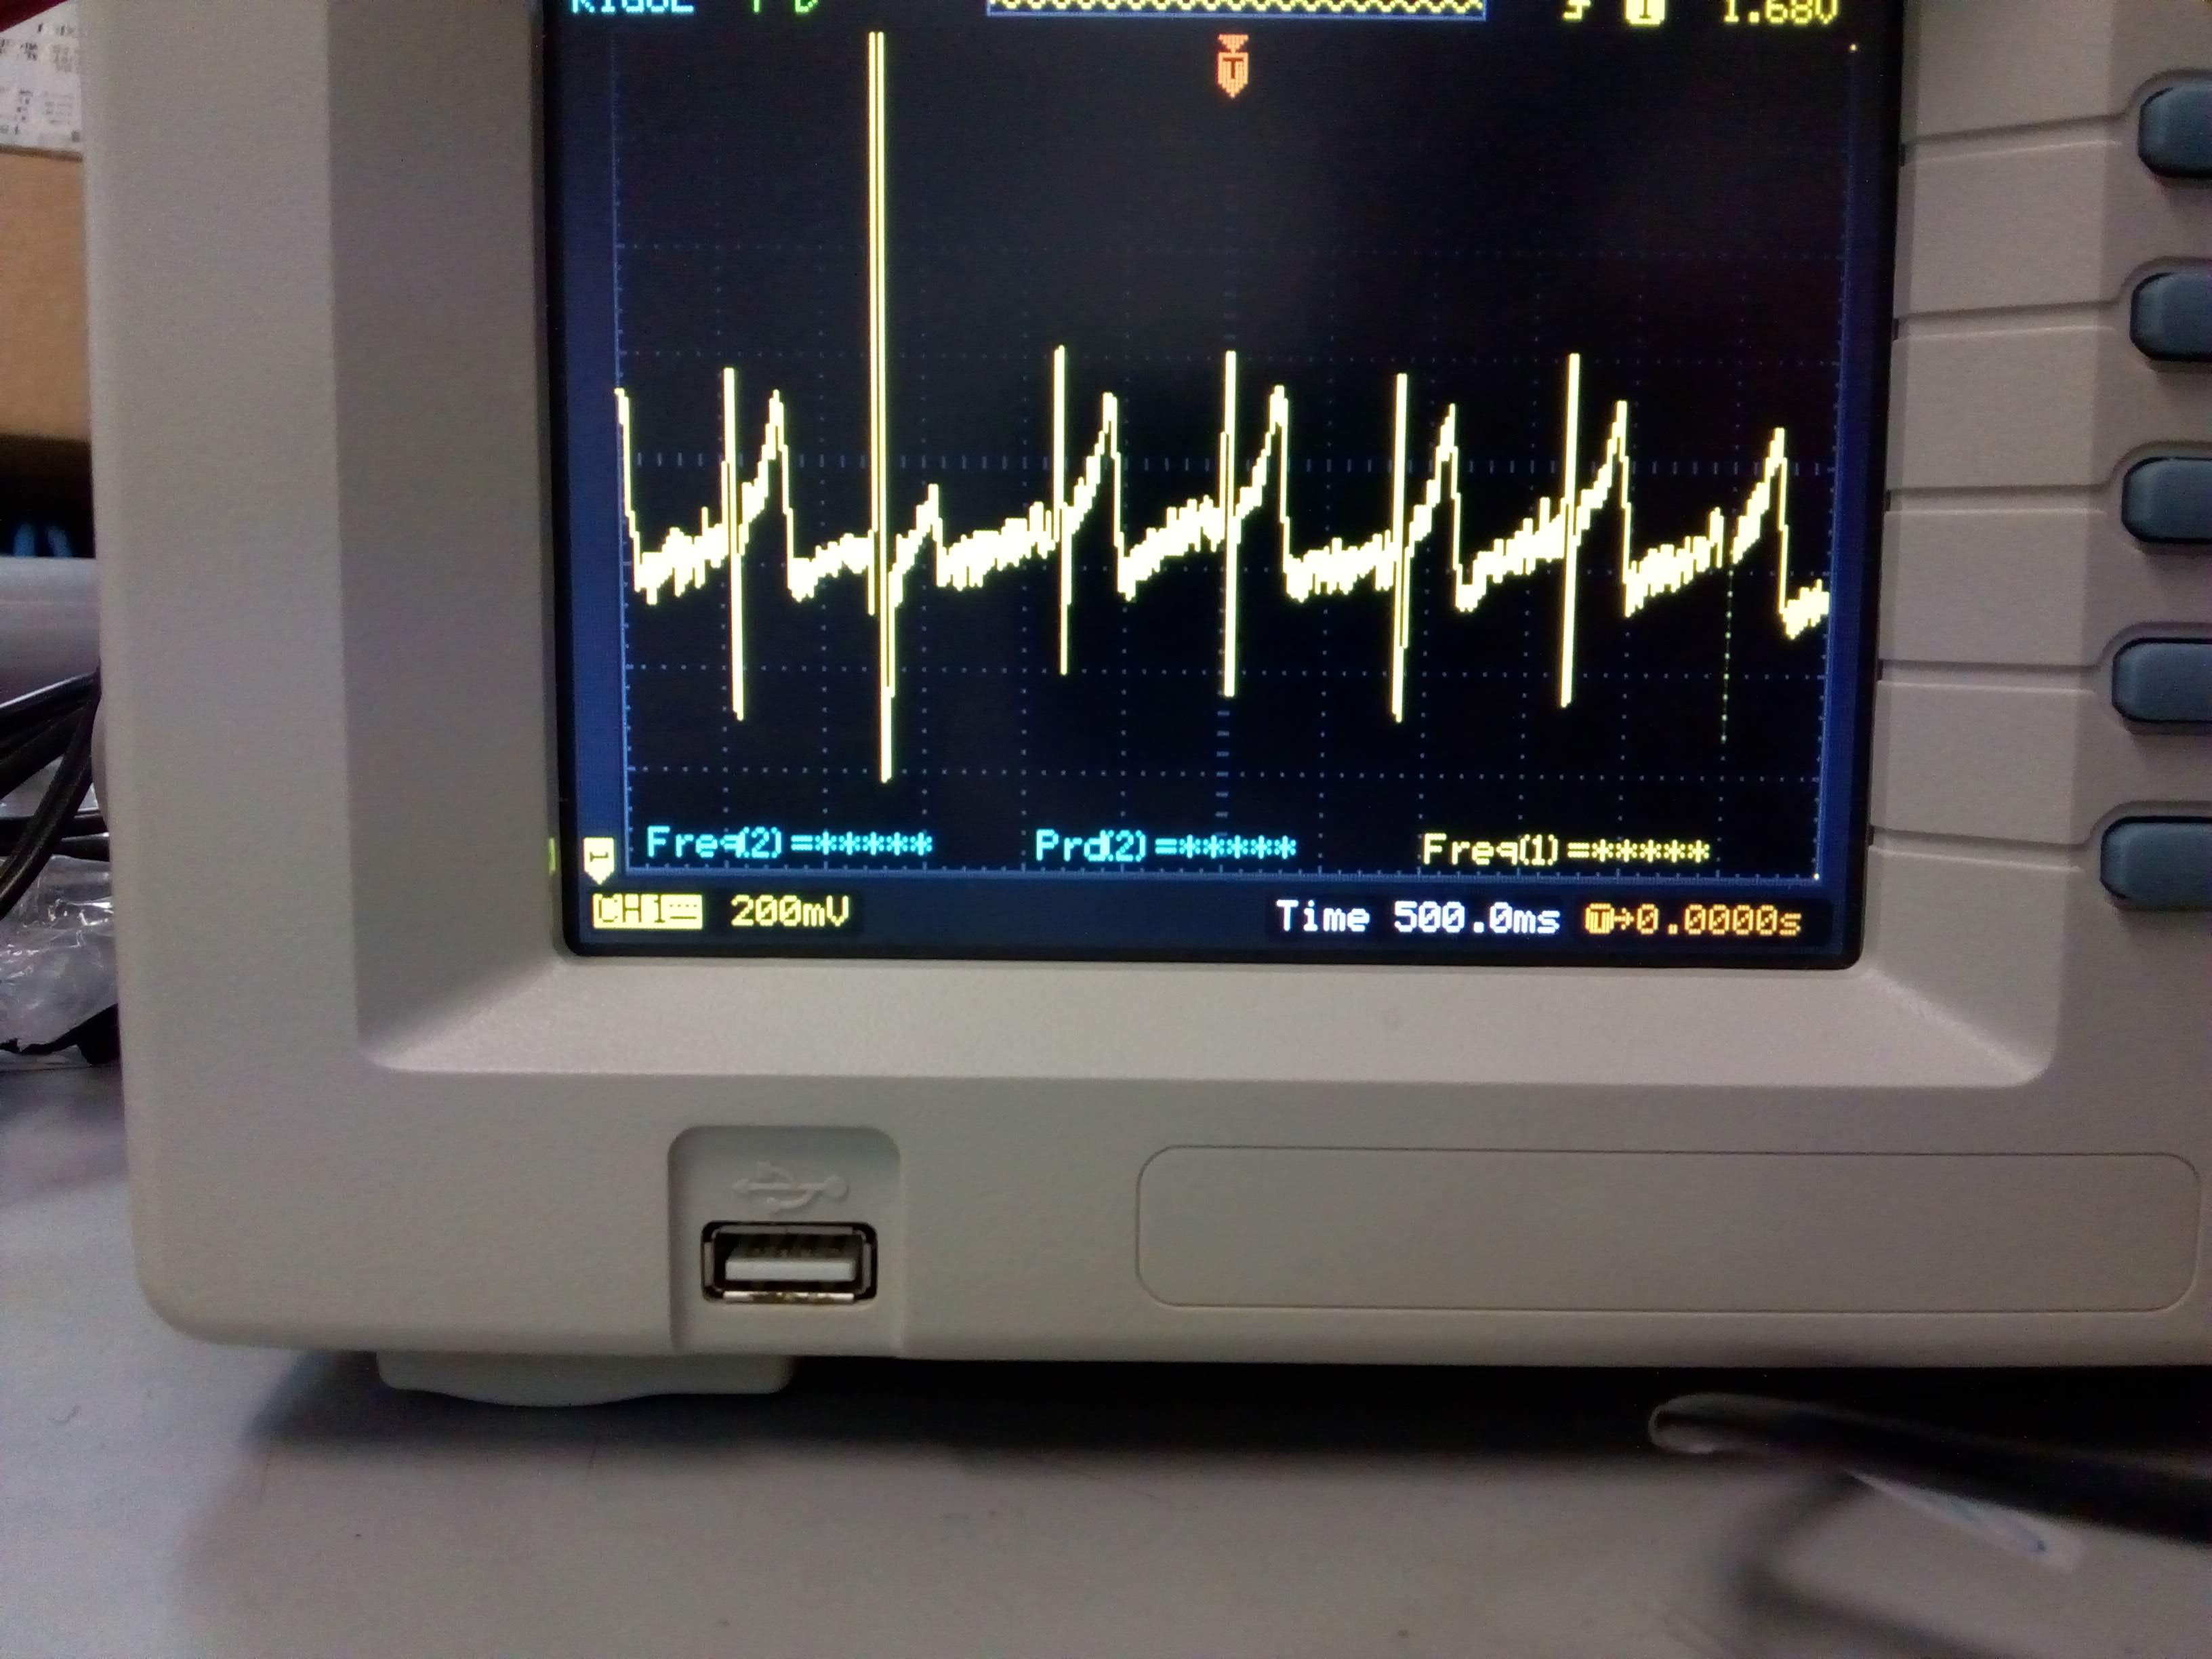
\includegraphics[width=0.8\textwidth]{AvancesPruebas/imagenes/AD8232-3.jpg}}
%	\caption{Señal analógica del sensor de pulso AD8232.}
%	\label{fig:AD8232Osciloscopio}
%\end{figure}

Se realizó una prueba unitaria para comprobar el correcto funcionamiento del sensor, así como para verificar que la señal analógica entregada por el mismo sea de utilidad para calcular la frecuencia cardíaca del paciente. El sensor fue alimentado con 3.3V mediante mediante el módulo FT232 a través de las terminales correspondientes en el sensor. En la figura \ref{fig:PulseSensor2} se muestra el sensor alimentado.\\

\begin{figure}[htbp!]
	\centering
	\fbox{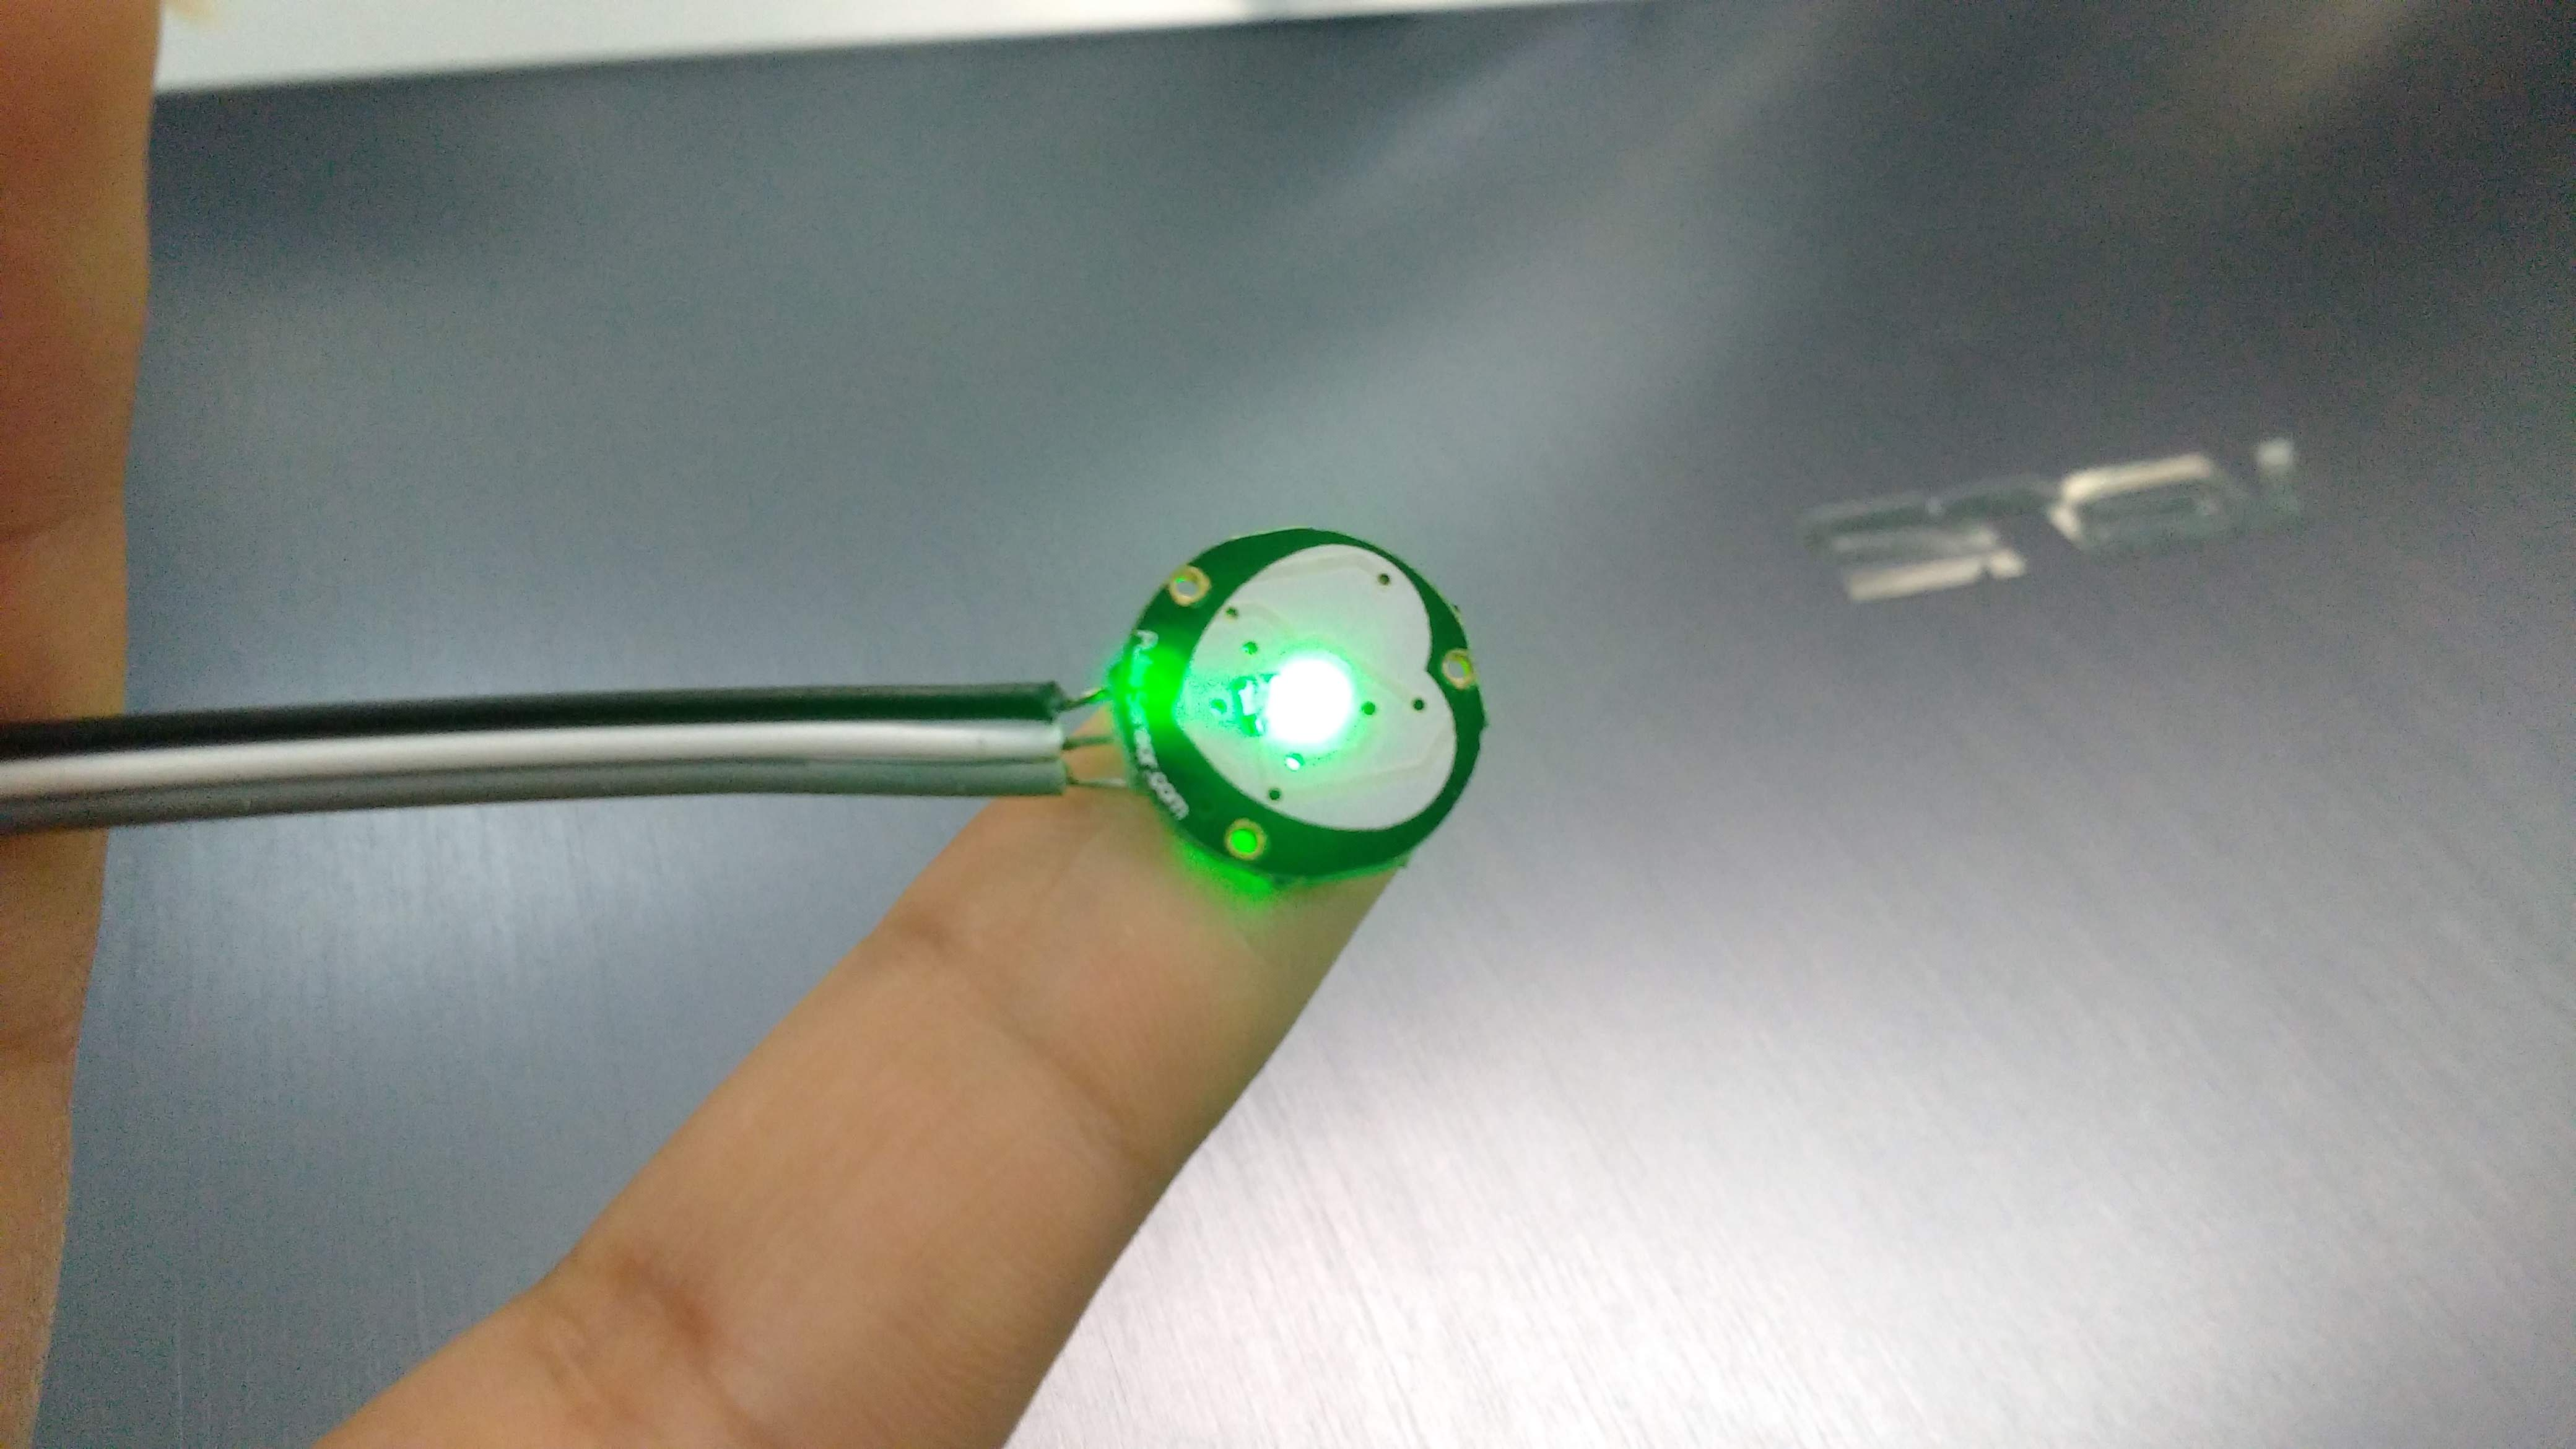
\includegraphics[width=0.8\textwidth]{AvancesPruebas/imagenes/PulseSensor2.jpg}}
	\caption{Sensor de pulso Pulse Sensor.}
	\label{fig:PulseSensor2}
\end{figure}

Debido a que el sensor es de tipo fotopletismógrafo, fue necesario aislarlo de luz externa que podría ocasionar alguna interferencia. Para lograr esto, se colocó el sensor de pulso en el dedo índice de la mano y se cubrió con un velcro negro, tal y como se muestra en la figura \ref{fig:PulseSensor1}.\\

\begin{figure}[htbp!]
	\centering
	\fbox{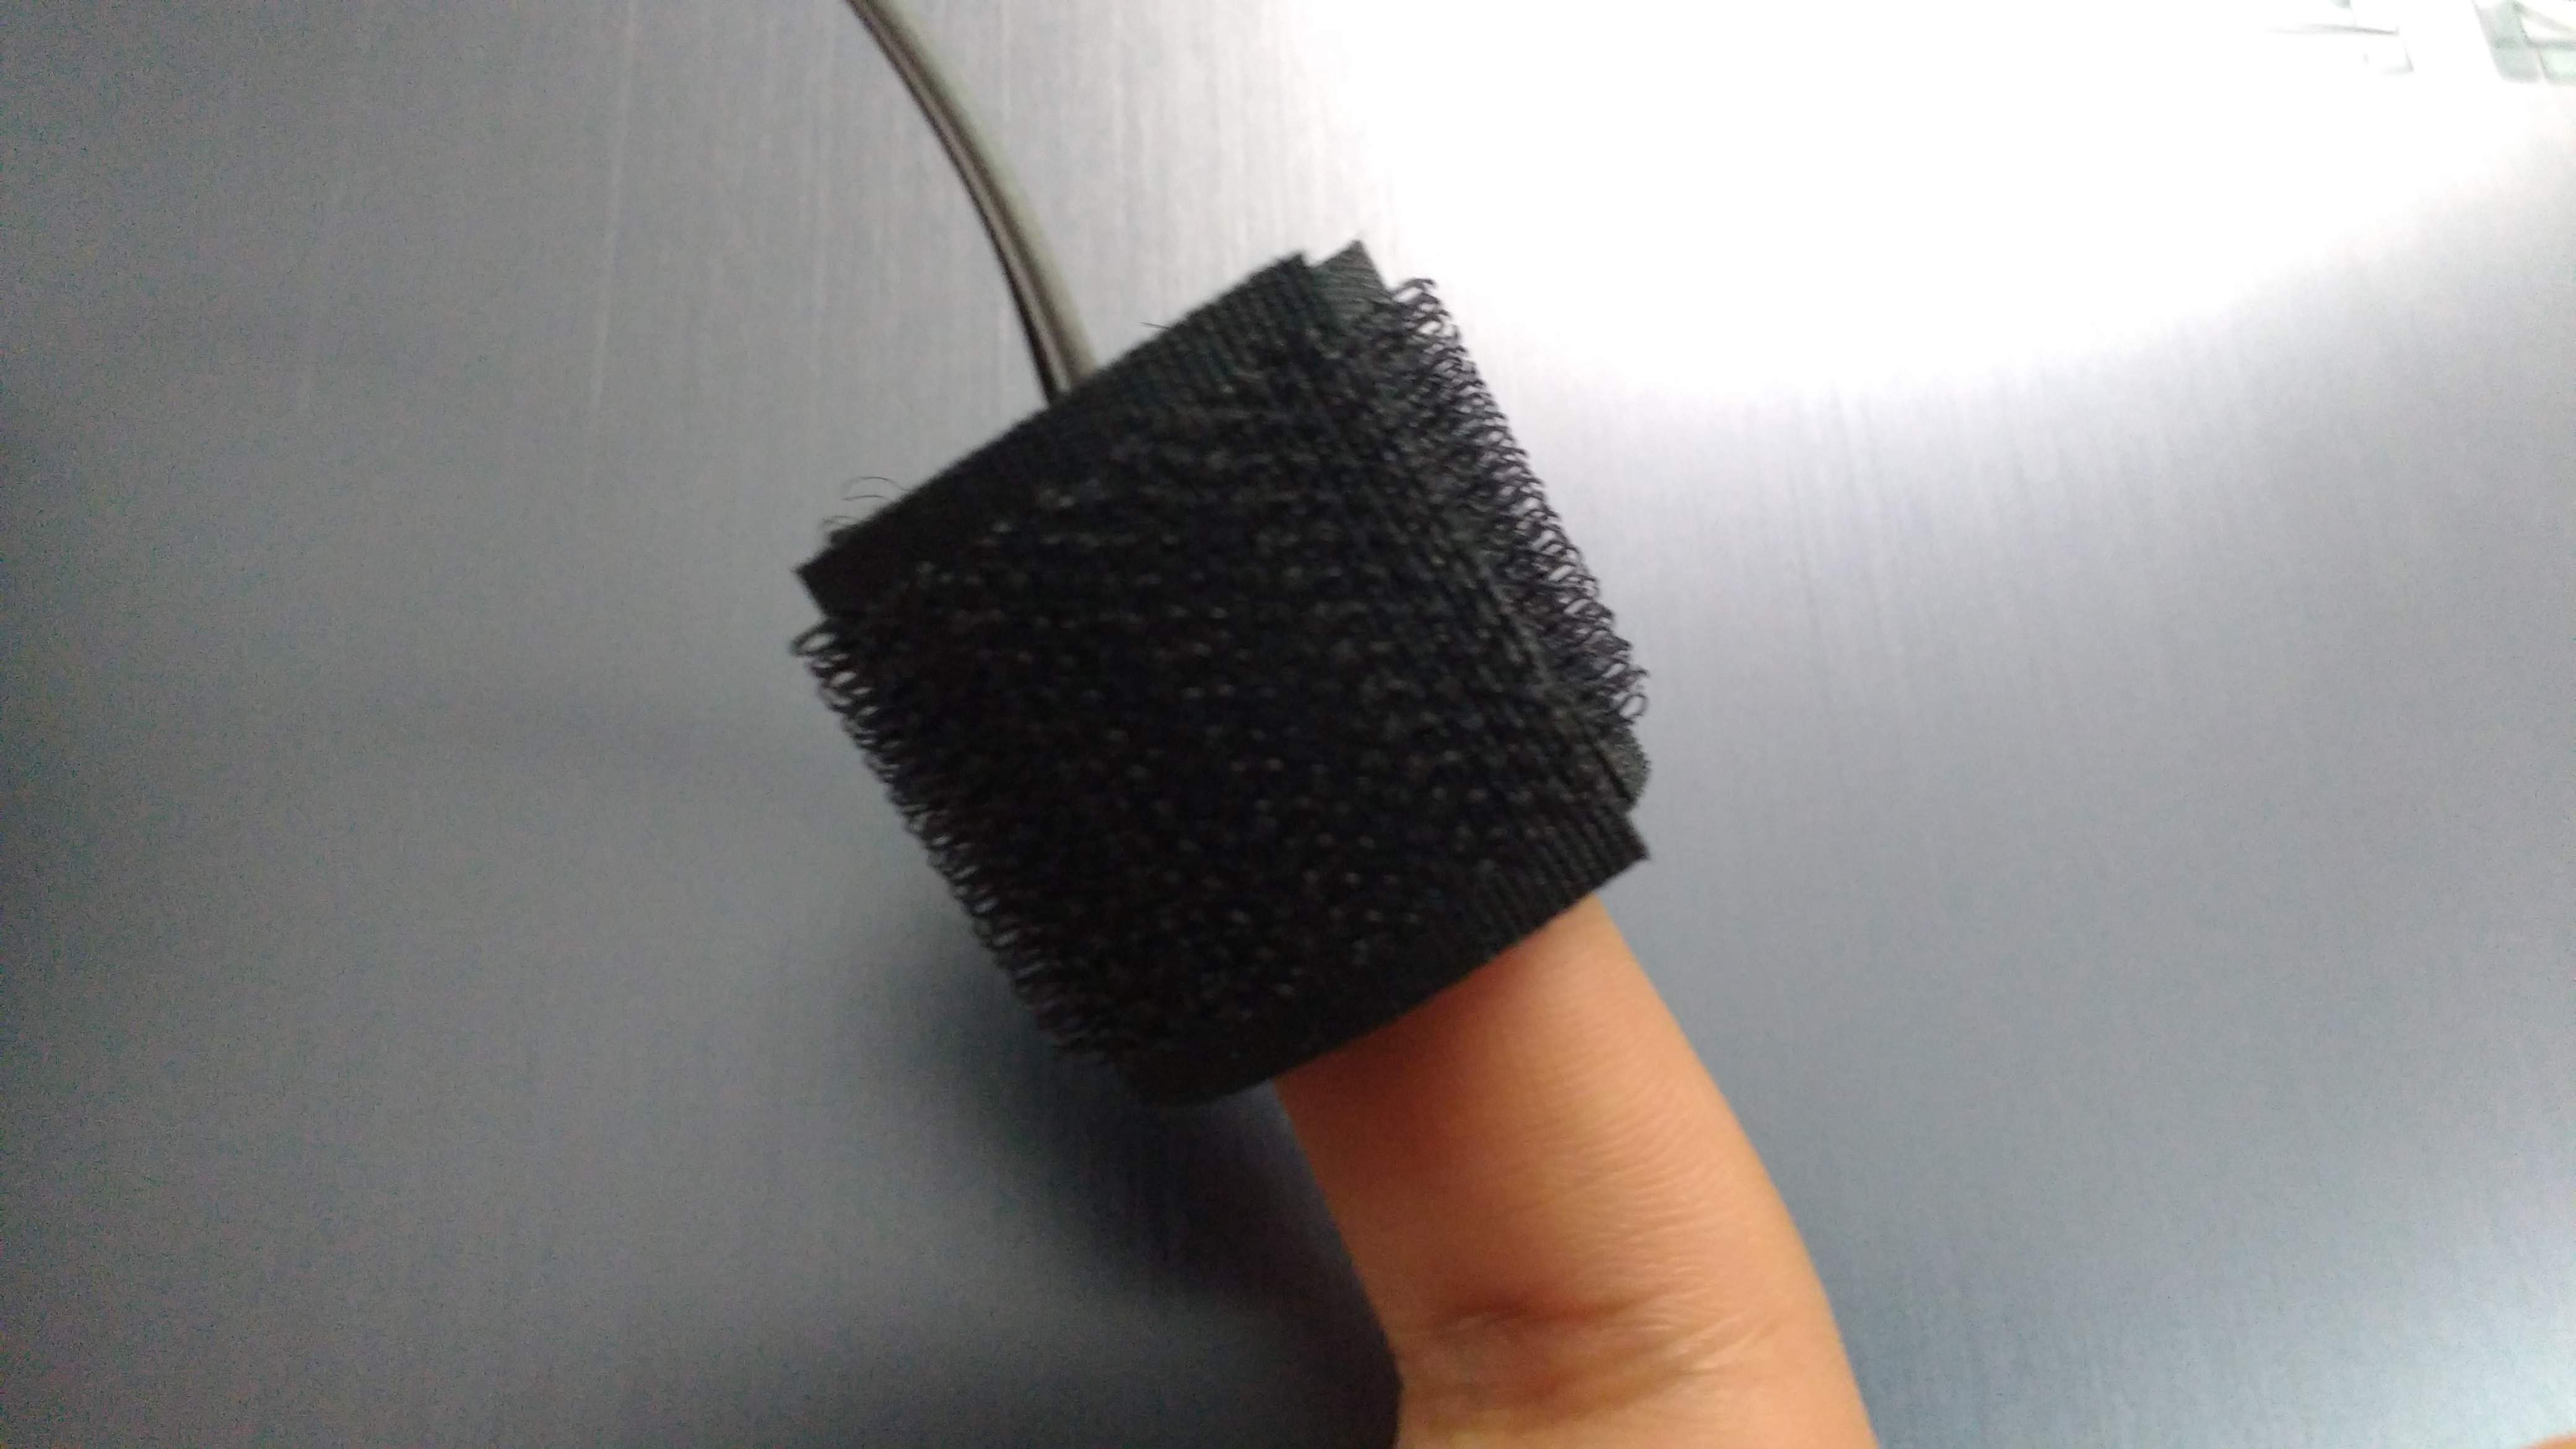
\includegraphics[width=0.8\textwidth]{AvancesPruebas/imagenes/PulseSensor1.jpg}}
	\caption{Prueba del sensor Pulse Sensor.}
	\label{fig:PulseSensor1}
\end{figure}

La señal obtenida de este sensor se muestra en el osciloscópio en la figura \ref{fig:PulseSensor3}.\\

\begin{figure}[htbp!]
	\centering
	\fbox{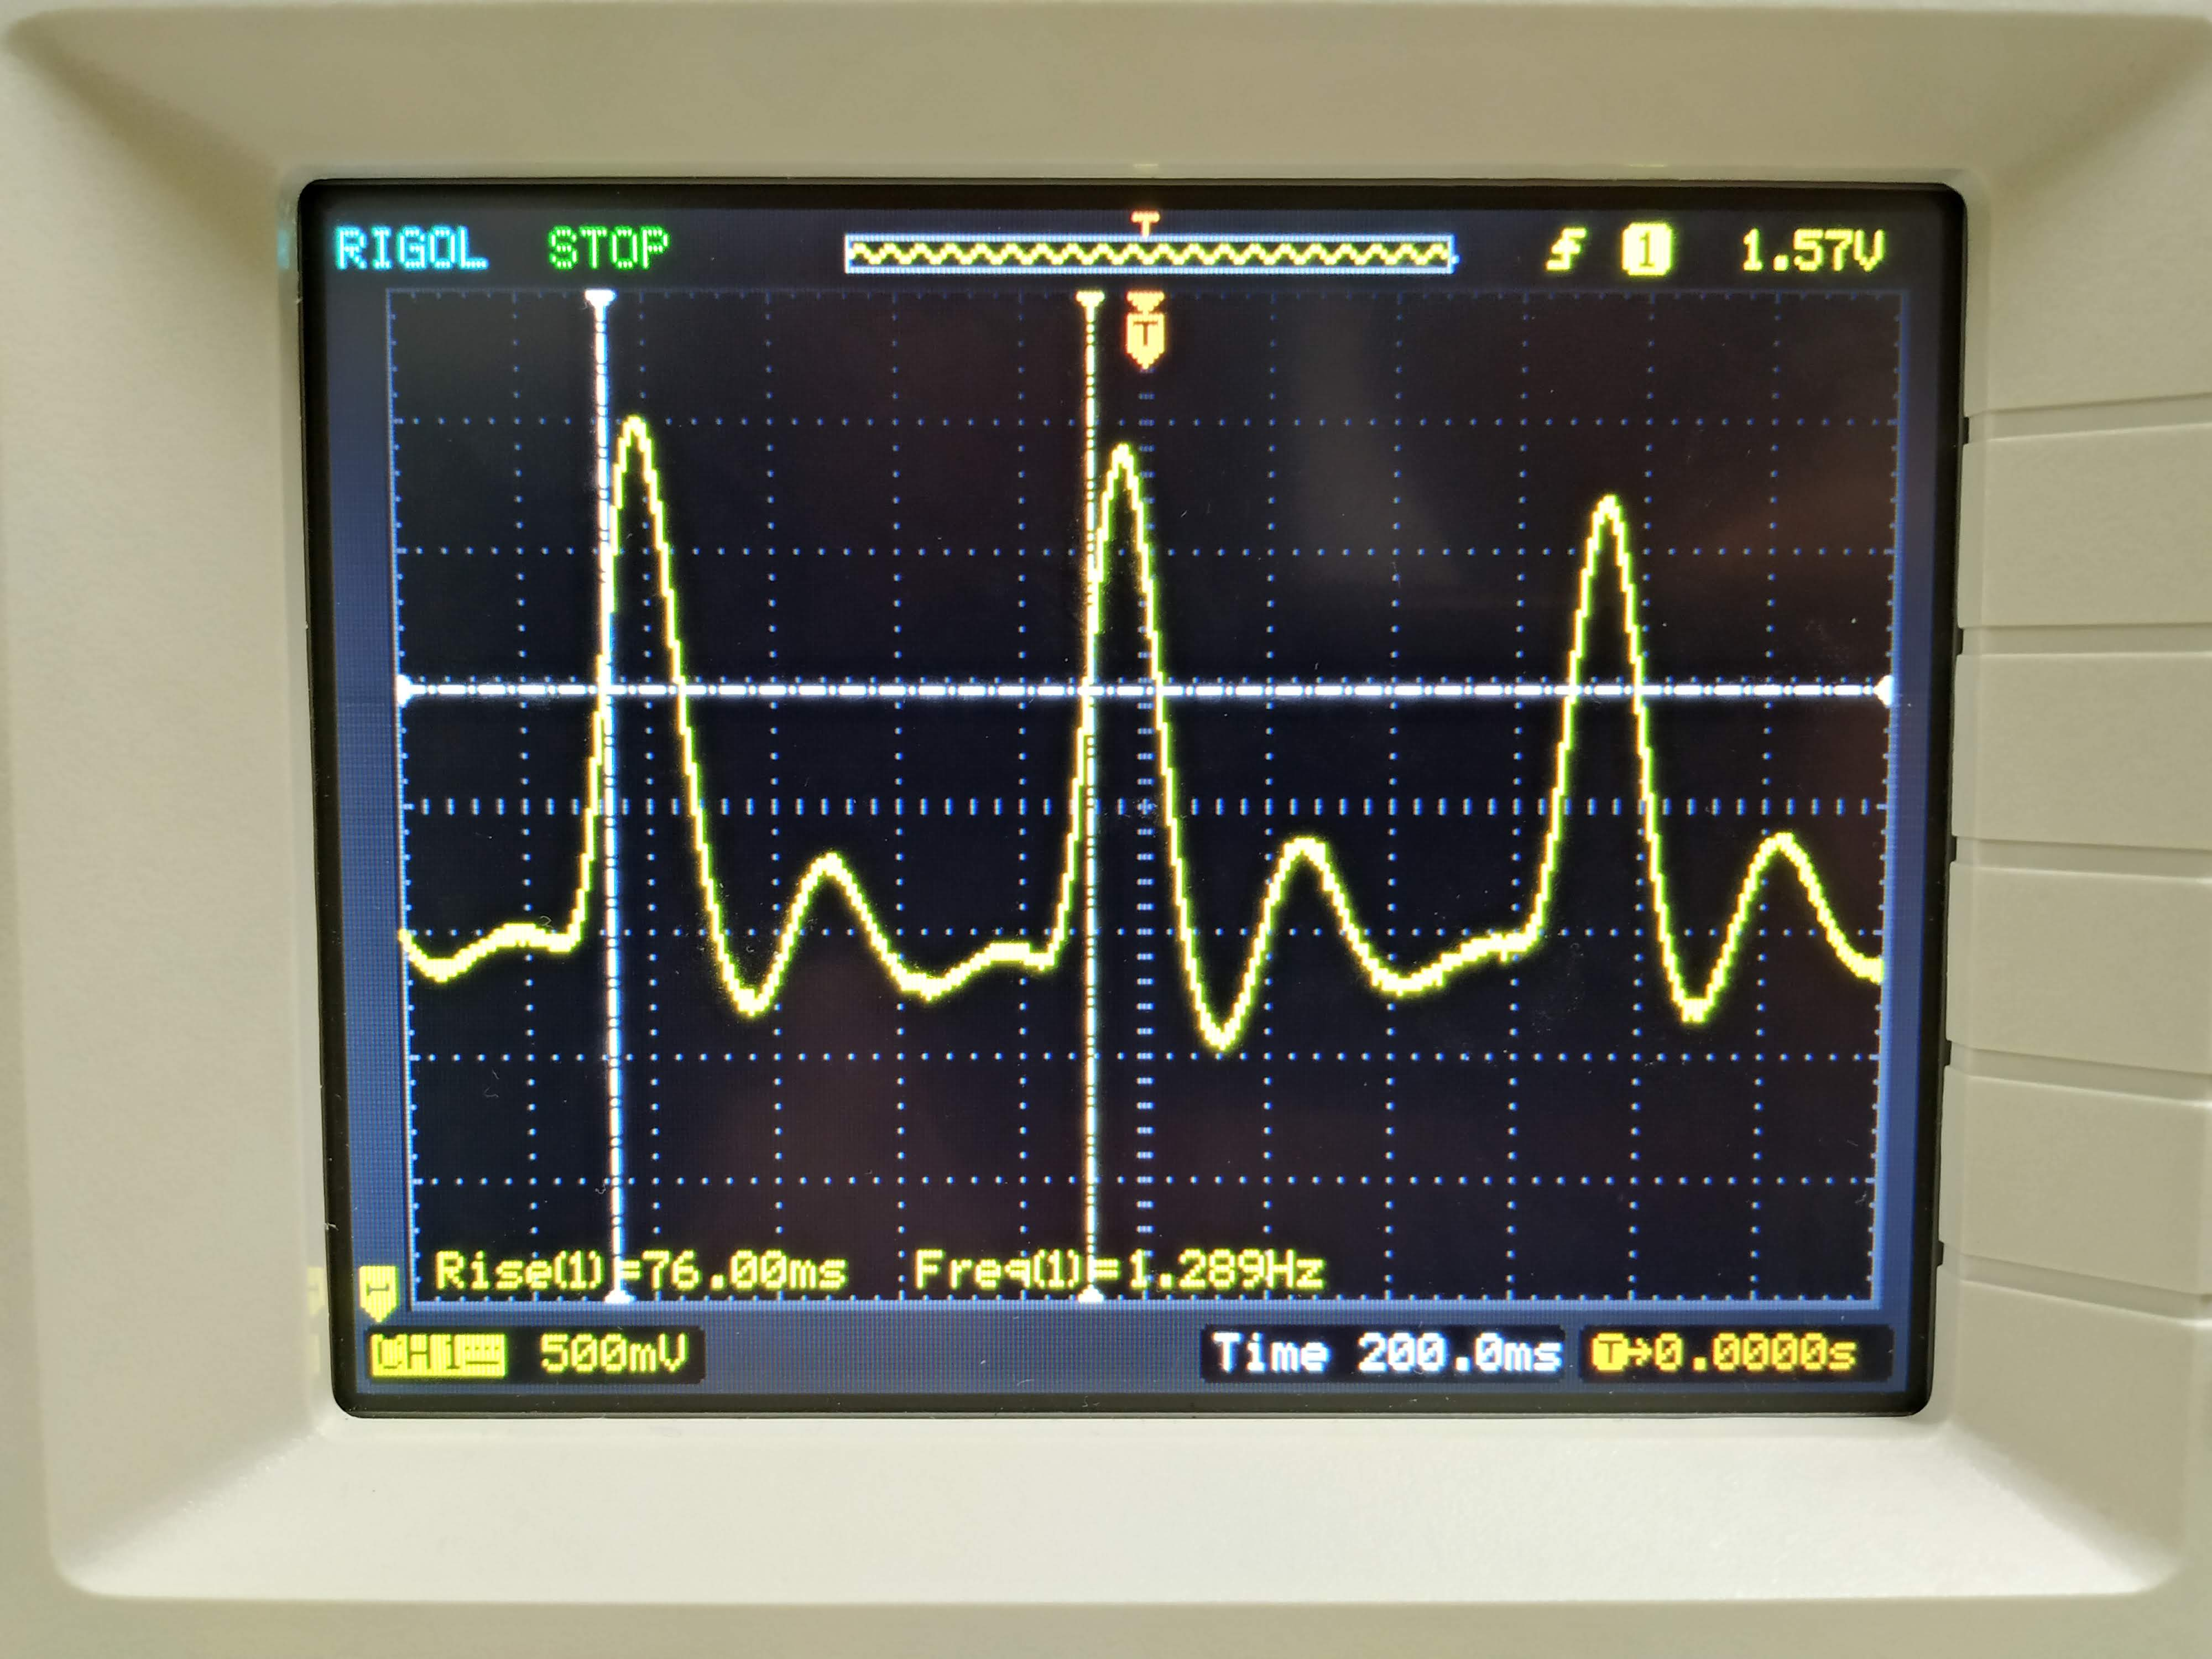
\includegraphics[width=0.8\textwidth]{AvancesPruebas/imagenes/PulseSensor3.jpg}}
	\caption{Señal analógica del sensor Pulse Sensor.}
	\label{fig:PulseSensor3}
\end{figure}

Esta señal muestra picos definidos al momento en el que se realiza el pulso cardíaco.

%========================================================================
\newpage	
\subsection{Digitalización de señal}
En esta etapa se configuró el microcontrolador para obtener y digitalizar la señal del Pulse Sensor haciendo uso del ADC. \\

El sensor se conectó al microcontrolador para que la señal fuera procesada y transformada por el ADC, y también se conectaron las terminales V+ y V- a su correspondiente en el microcontrolador para ser alimentado con 3.3V, tal como se muestra en la figura \ref{fig:ConexionPulseSensor}. \\

\begin{figure}[htbp!]
	\centering
	\fbox{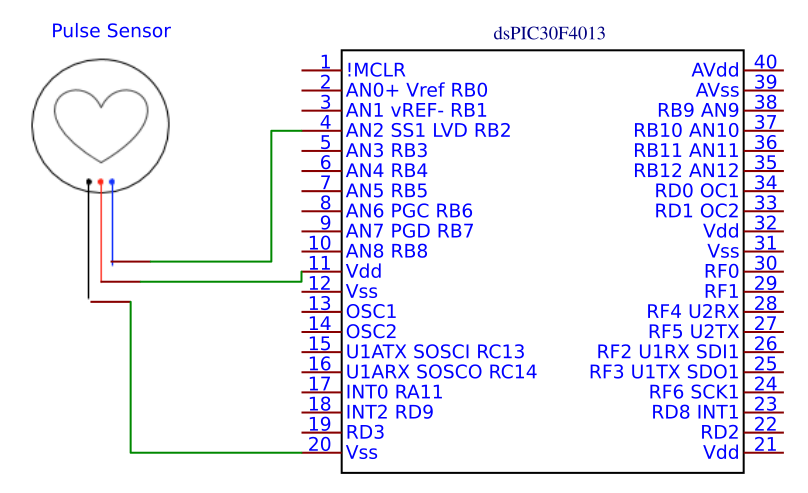
\includegraphics[width=0.7\textwidth]{AvancesPruebas/imagenes/PulseSensorConexion.png}}
	\caption{Diagrama de conexión del Pulse Sensor con el microcontrolador.}
	\label{fig:ConexionPulseSensor}
\end{figure}

En la figura \ref{fig:conexionPS} se muestra la conexión de estos elementos. \\

\begin{figure}[htbp!]
	\centering
	\fbox{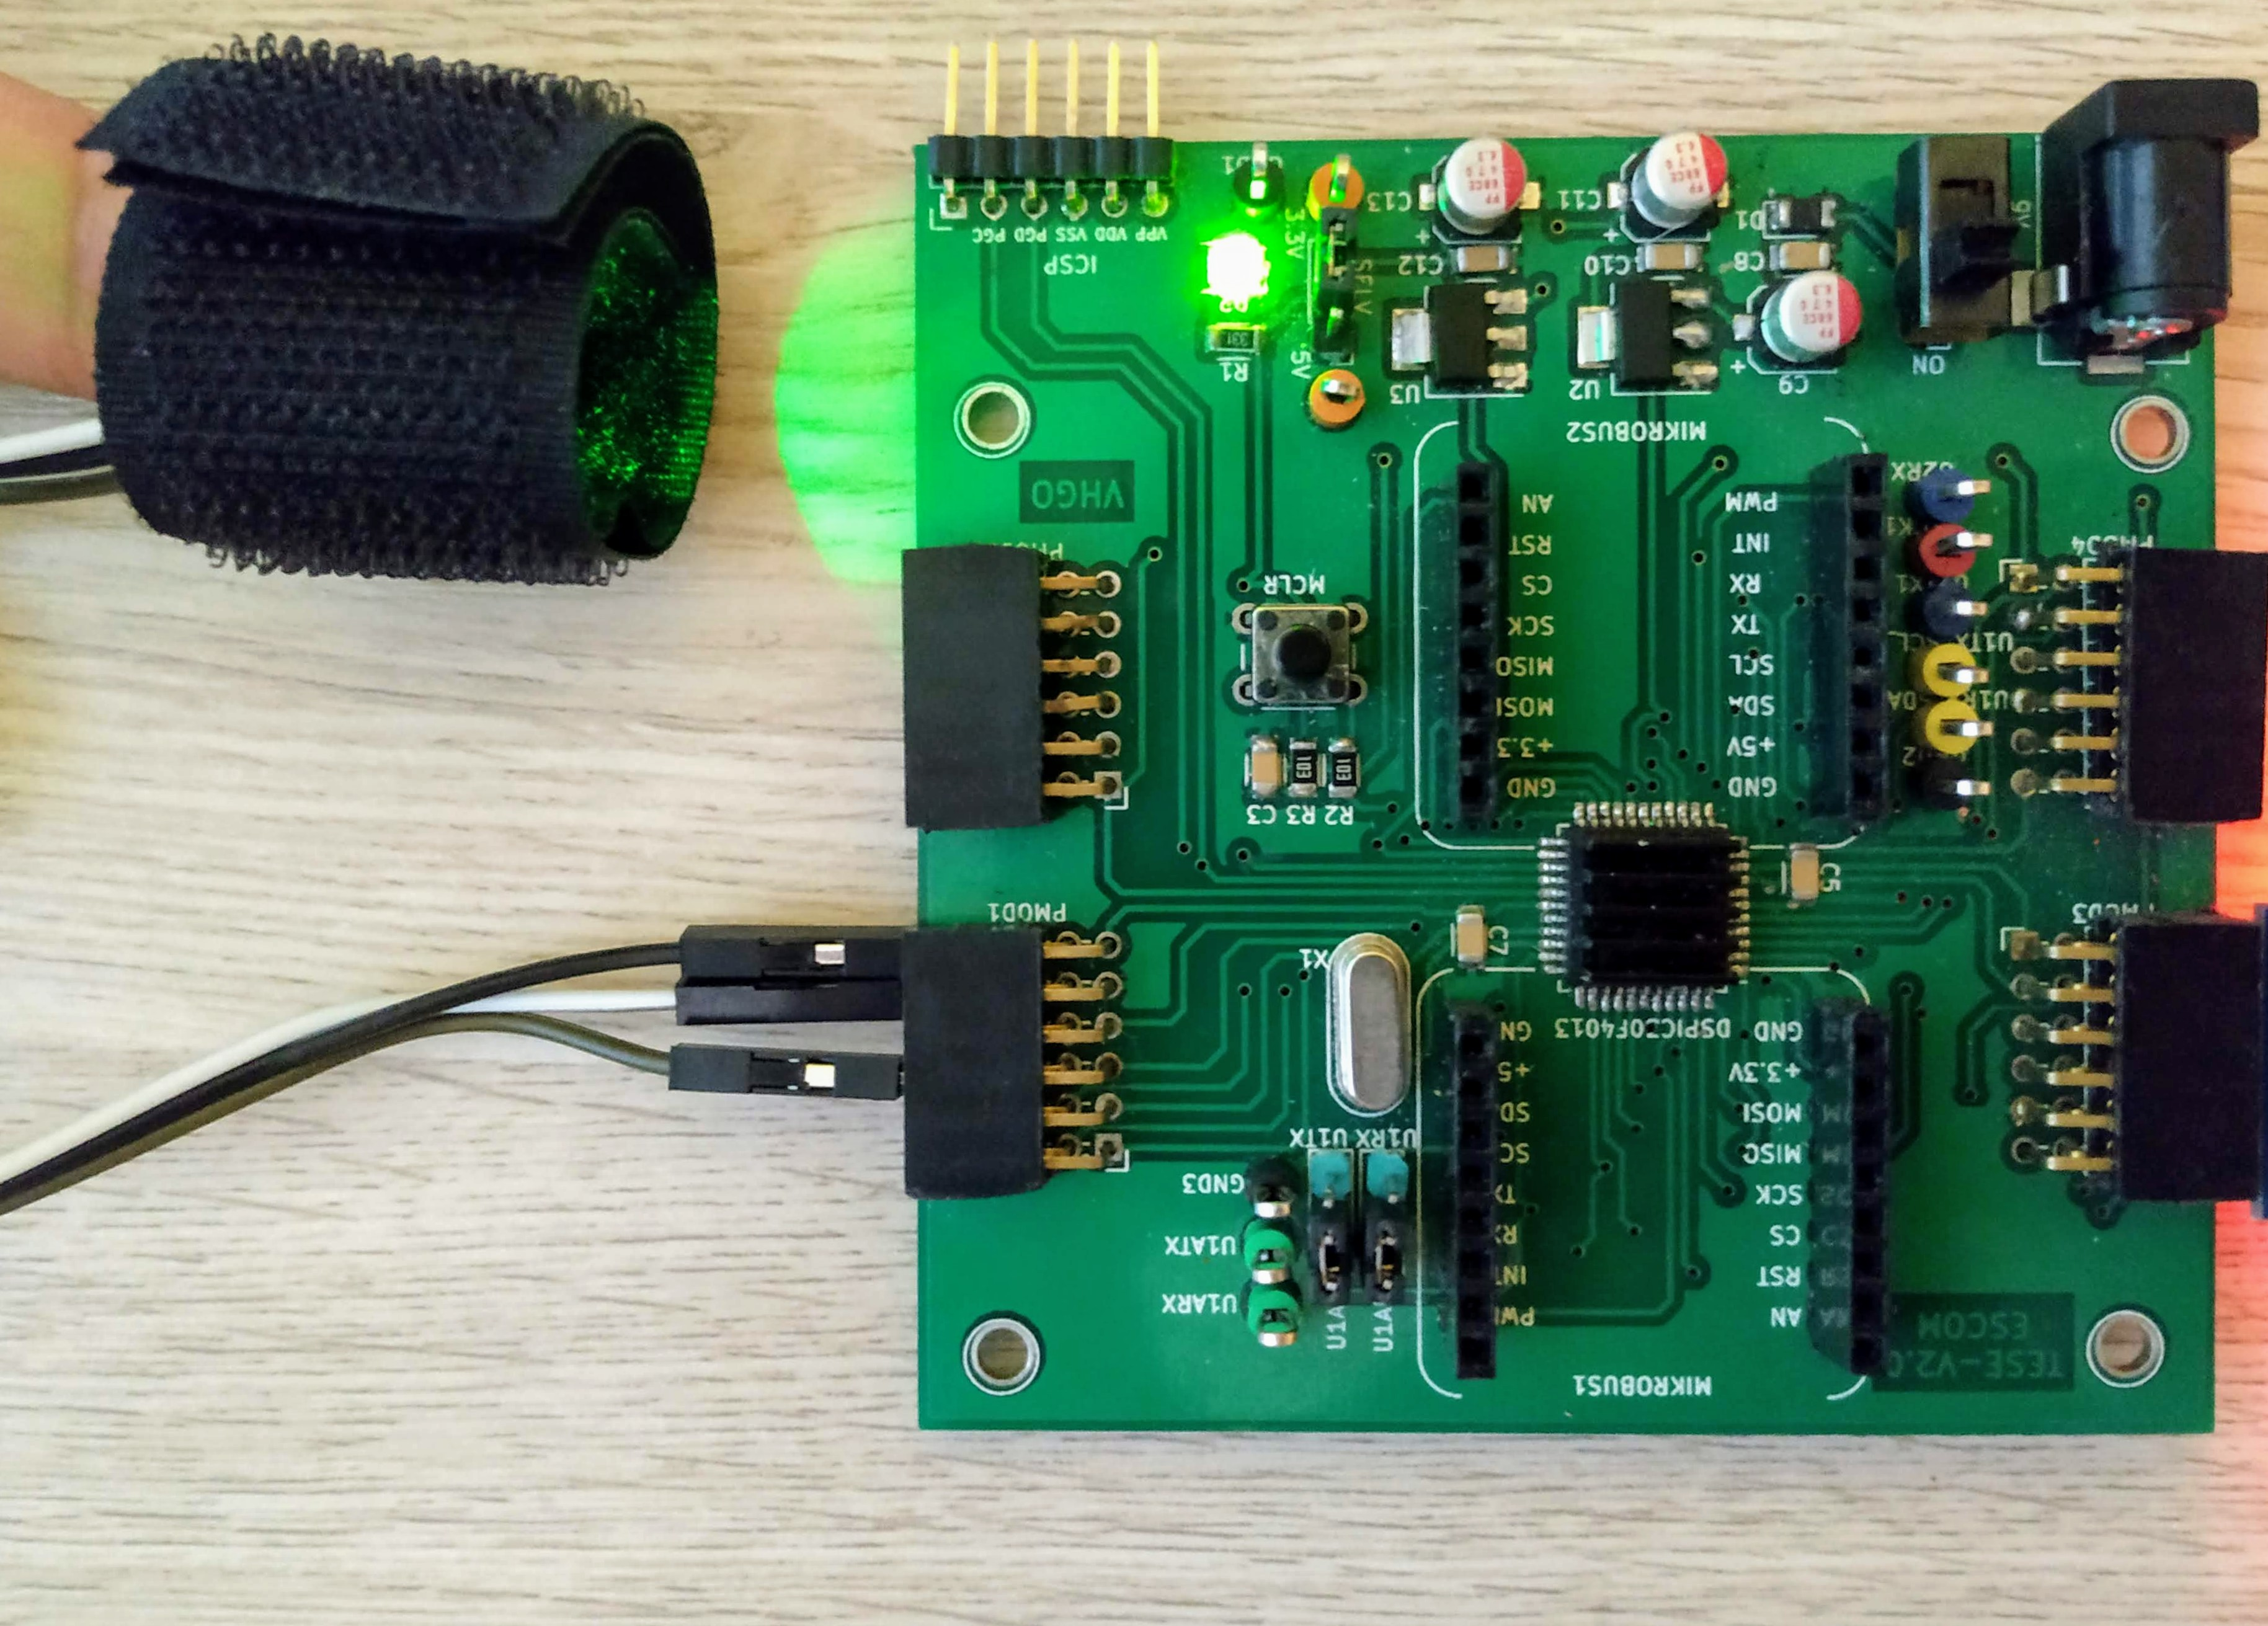
\includegraphics[width=0.8\textwidth]{AvancesPruebas/imagenes/conexionPS.jpg}}
	\caption{Conexión de Pulse Sensor con el microcontrolador.}
	\label{fig:conexionPS}
\end{figure}

En la figura \ref{fig:ConfiguracionMicro} se muestra el diagrama de flujo indicando los pasos realizados para la configuración de los puertos, ADC y UART del microcontrolador y así poder obtener y procesar la señal medida del sensor de pulso. \\

Para estas tareas se utilizó el oscilador interno del microcontrolador. \\

A continuación se describen las etapas del diagrama de flujo.

\begin{enumerate}
	\item \textbf{Configuración de puertos:} Esta rutina inicializa los periféricos del microcontrolador indicando qué puertos serán considerados como entradas o salidas. En este caso, las entradas que tendrá el microcontrolador son el pin B2,que funcionará como entrada analógica (AN2) para la salida del sensor de pulso y el pin C14 el cuál es el transmisor TX del UART. Para el caso de las salidas, se configuró el pin C13 el cual es el receptor del UART. 
	
%	\item \textbf{Configuración de reloj para ADC:} Se configura el
	
	\item \textbf{Configuración UART:} Esta rutina configura el UART a una taza de transferencia de 19200 baudios e indica los pines a utilizar. También se incluyen las interrupciones correspondientes al UART.
	
	\item \textbf{Configuración de ADC:} En esta sección se especifica que el pin de entrada B2 será el canal de entrada analógico (AN2) para el ADC. Se utilizó una frecuencia de muestreo de $512\ Hz$ por lo que se realizó la configuración del Timer 3 para el control del ADC. También se especificó la interrupción del ADC para enviar el valor digital al UART. 
	
\end{enumerate}

	\begin{figure}[htbp!]
		\centering
		\fbox{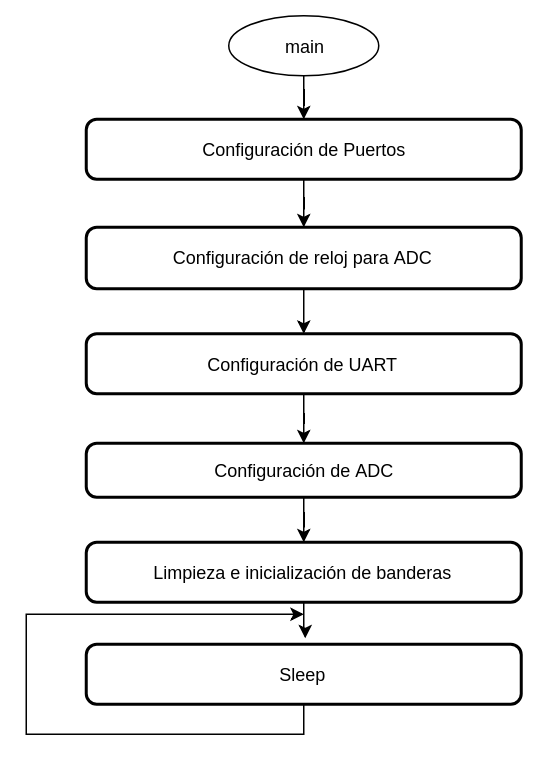
\includegraphics[width=0.6\textwidth]{AvancesPruebas/imagenes/ConfiguracionMicro.png}}
		\caption{Diagrama de flujo del programa de configuración del dsPIC30F4013.}
		\label{fig:ConfiguracionMicro}
	\end{figure}

En esta etapa se realizó un programas en lenguaje C para obtener los valores de la señal digital enviados a través del módulo FT232.

En la figura \ref{fig:FlujoSerial} se muestra el diagrama de flujo para la obtención de los datos digitalizados por el ADC y el proceso llevado a cabo para graficar los datos obtenidos.\\

A continuación se describen las etapas del diagrama de flujo realizado para esta función.
\begin{enumerate}
	\item \textbf{Configuración de interfaz serie:} Esta función configura los elementos de la interfaz serie como el nombre del dispositivo serial a usar y la taza de transferencia en baudios.
	\item \textbf{Creación/apertura de archivo:} En este paso se crea o abre un archivo en el cuál se almacenarán los datos leídos a través de la interfaz serie.
	\item \textbf{Obtención de datos de la interfaz serie:} Lee los datos que están siendo enviados por UART a través de la interfaz serie configurada anteriormente.
	\item \textbf{Cierre de archivo:} Una vez leídos todos los datos por UART, se cierra el archivo en donde se realizó la escritura de los mismos.
	\item \textbf{Gráfica de señal digitalizada:} Se muestra una gráfica a partir del archivo creado usando el programa gnuplot, en donde puede verse la señal resultante.
\end{enumerate}

	\begin{figure}[htbp!]
		\centering
		\fbox{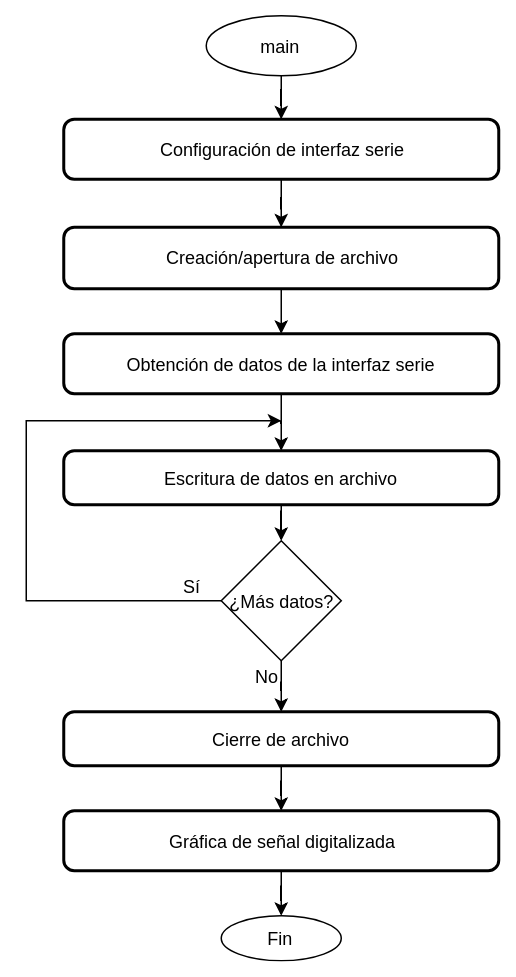
\includegraphics[width=0.6\textwidth]{AvancesPruebas/imagenes/Serial.png}}
		\caption{Diagrama de flujo de la obtención de señal digitalizada.}
		\label{fig:FlujoSerial}
	\end{figure}
%\pagebreak
\newpage		


%\subsubsection{AD8232}
%El primer sensor que fue conectado fue el AD8232, el diagrama de conexión se muestra en la figura \ref{fig:ConexionAD8232}. En ella se puede observar que la única entrada que tiene el microcontrolador para esta prueba es en el pin B2, el cual es tomado como entrada analógica y es de donde el ADC tomará los datos para convertirlos.\\
%
%Es importante aclarar que este sensor fue alimentado con 3.3 V.\\
%
%	\begin{figure}[htbp!]
%		\centering
%		\fbox{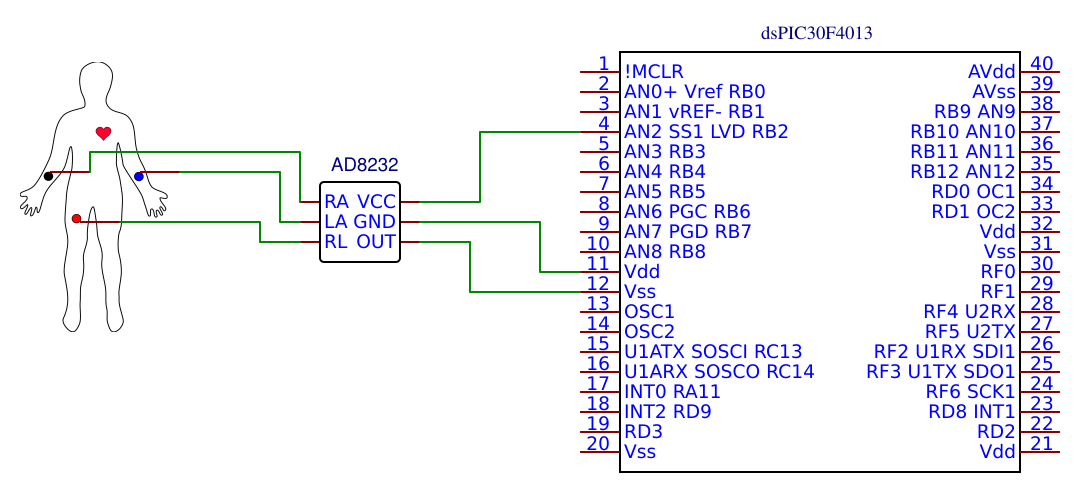
\includegraphics[width=0.95\textwidth]{AvancesPruebas/imagenes/AD8232Conexion.png}}
%		\caption{Conexión de AD8232 con dsPIC30F4013.}
%		\label{fig:ConexionAD8232}
%	\end{figure}
%	
%El resultado de la ejecución, así como la gráfica obtenida de la señal digital se muestran en las figuras \ref{fig:TerminalAD8232} y \ref{fig:GraficaAD8232} respectivamente.\\
%
%	\begin{figure}[htbp!]
%		\centering
%		\fbox{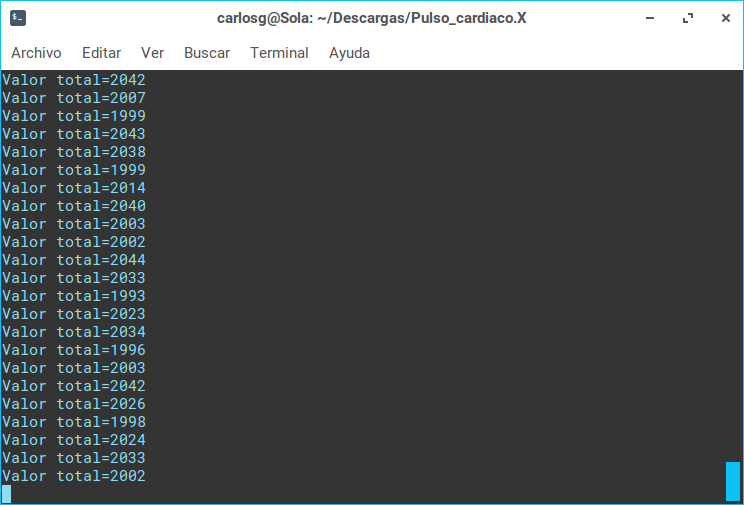
\includegraphics[width=0.6\textwidth]{AvancesPruebas/imagenes/terminalAD8232.png}}
%		\caption{Resultado de ejecución para sensor AD8232.}
%		\label{fig:TerminalAD8232}
%	\end{figure}
%	
%	\begin{figure}[htbp!]
%		\centering
%		\fbox{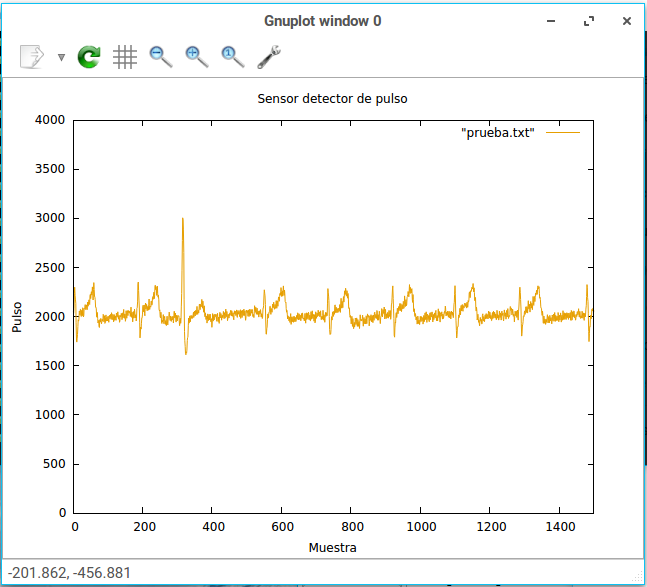
\includegraphics[width=0.6\textwidth]{AvancesPruebas/imagenes/graficaAD8232.png}}
%		\caption{Gráfica de señal del sensor AD8232.}
%		\label{fig:GraficaAD8232}
%	\end{figure}
%	
%	
%\subsubsection{Pulse Sensor}	

En las figuras  \ref{fig:TerminalPulseSensor} y \ref{fig:GraficaPulseSensor} se muestra el resultado de la digitalización de la señal en la computadora.
	
	\begin{figure}[htbp!]
		\centering
		\fbox{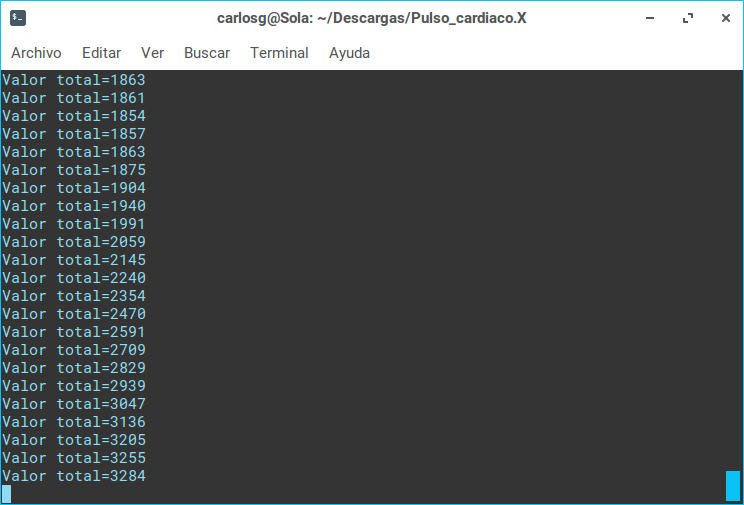
\includegraphics[width=0.9\textwidth]{AvancesPruebas/imagenes/terminalPulseSensor.png}}
		\caption{Resultado de ejecución para sensor Pulse Sensor.}
		\label{fig:TerminalPulseSensor}
	\end{figure}
	
	\begin{figure}[htbp!]
		\centering
		\fbox{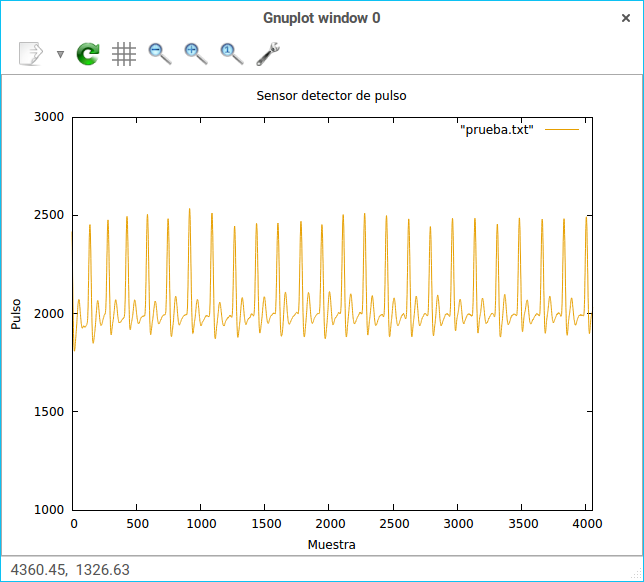
\includegraphics[width=0.8\textwidth]{AvancesPruebas/imagenes/graficaPulseSensor.png}}
		\caption{Gráfica de señal del sensor Pulse Sensor.}
		\label{fig:GraficaPulseSensor}
	\end{figure}
	
%========================================================================
\subsection{Procesamiento digital de señal}
En esta etapa se realizó el procesamiento digital de la señal obtenida en el paso anterior, mediante la aplicación del algoritmo de autocorrelación y la búsqueda del valor máximo para obtener la frecuencia fundamental de la señal y calcular la frecuencia cardíaca.\\

Después de haber verificado el funcionamiento del sensor y haber obtenido exitosamente la señal digital desde el ADC del microcontrolador, se procedió a definir la frecuencia de muestreo. Para definir esta frecuencia se tiene del teorema de Nyquist ($Fs \geq 2f$). Considerando una frecuencia cardíaca de $210\ lpm$, se tiene que $Fs \geq 7.3332\ Hz$, pero se redondeó a $8\ Hz$ para trabajar con un valor entero. Por lo tanto frecuencias mayores a partir de $8\ Hz$ serían adecuadas para obtener la información necesaria para el tratamiento de la señal digital.\\

Para el cálculo de la frecuencia cardíaca se utilizó la ecuación dada por:
\begin{equation}
\label{eq:lpm}
lpm = \frac{Fs}{pos} * 60
\end{equation}

donde:
\begin{itemize}
	\item $lpm$: frecuencia cardíaca expresada en latidos por minuto.
	\item $Fs$: frecuencia de muestreo.
	\item $pos$: índice de la posición del segundo valor máximo de la autocorrelación.\\
\end{itemize}

Dado que la fórmula (\ref{eq:lpm}) depende de la frecuencia de muestreo ($Fs$) y la posición del valor máximo de la autocorrelación ($pos$), se realizaron pruebas variando esta frecuencia desde $8\ Hz$ hasta $512\ Hz$. \\

En la tabla \ref{sensorPulso:resultadosCalculoFs} se muestra un resumen de los resultados obtenidos al aplicar la fórmula anterior a las frecuencias mencionadas con el fin de obtener los resultados posibles de la frecuencia cardíaca expresada en latidos por minuto.

\begin{table}[htbp]
	\begin{center}
		\begin{tabular}{|l|l|l|l|l|l|l|}
			\hline
			\textbf{pos / Fs} & \textbf{8 Hz} & \textbf{16 Hz} & \textbf{...} & \textbf{128 Hz} & \textbf{...} & \textbf{512 Hz} \\
			\hline \hline
			\textbf{3} & 160 & 320 & ... & 2560 & ... & 10240 \\
			\hline
			\textbf{4} & 120 & 240 & ... & 1920 & ... & 7680 \\
			\hline
			\textbf{5} & 96 & 192 & ... & 1536 & ... & 6144 \\
			\hline
			\textbf{...} & ... & ... & ... & ... & ... & ...  \\
			\hline
			\textbf{83} & 5.783 & 11.566 & ... & 92.530 & ... & 370.120 \\
			\hline
			\textbf{84} & 5.714 & 11.429 & ... & 91.429 & ... & 365.714 \\
			\hline
			\textbf{85} & 5.647 & 11.294 & ... & 90.353 & ... & 361.412 \\
			\hline
			\textbf{86} & 5.581 & 11.163 & ... & 89.302 & ... & 357.209 \\
			\hline
			\textbf{87} & 5.517 & 11.034 & ... & 88.276 & ... & 353.103 \\
			\hline
			\textbf{...} & ... & ... & ... & ... & ... & ...  \\
			\hline
			\textbf{148} & 3.243 & 6.486 & ... & 51.892 & ... & 207.568 \\
			\hline
			\textbf{149} & 3.221 & 6.443 & ... & 51.544 & ... & 206.174 \\
			\hline
			\textbf{150} & 3.2 & 6.4 & ... & 51.2 & ... & 204.8 \\
			\hline
		\end{tabular}
		\caption{Cálculo de frecuencia cardíaca.}
		\label{sensorPulso:resultadosCalculoFs}
	\end{center}
\end{table}

De los resultados mostrados en la tabla  \ref{sensorPulso:resultadosCalculoFs}, se observó que a menor $Fs$, más amplio es el rango de valores faltantes, por ejemplo, a $8\ Hz$ no se encuentran valores entre los $120$ y $96\ lpm$, lo que sucede con todas las frecuencias consideradas en ciertos valores, sin embargo, se determinó que para la frecuencia de $128\ Hz$ se tenía un rango de valores continuos hasta los $94\ lpm$ y con un rango de error de $0.84\%$ hasta $120\ lpm$, permitiendo tener una aproximación de los valores esperados sin sobrepasar la memoria de datos del microcontrolador de 2 KB. \\

Para realizar el cálculo de la frecuencia cardíaca se implementó un algoritmo para obtener la autocorrelación de la señal. La ecuación está dada por:

\begin{equation}
\label{eq:autocorr}
Cxx[n] = \frac{1}{N} \sum_{m=0}^{N-1-n}x[m]x[m+n]
\end{equation}

donde: 
\begin{itemize}
	\item $Cxx$: valor de la autocorrelación para un punto un particular.
	\item $n$: índice del arreglo de autocorrelación.
	\item $m$: índice del arreglo de la señal digital.
	\item $N$: cantidad de muestras para la autocorrelación.\\
\end{itemize}

Para definir la cantidad de muestras ($N$) necesarias para obtener el resultado de la autocorrelación, se realizaron 80 pruebas en las que se digitalizaron $4096$ valores utilizando el ADC del microcontrolador y se procesaron con un programa en C, en el que se aplicaba el algoritmo de autocorrelación considerando $16$ muestras y hasta $4096$, aumentando $16$ muestras para cada cálculo. Con esto se determinó el error porcentual de los resultados comparados con las mediciones reales de la frecuencia cardíaca obtenida con el método de palpación. \\

De esos resultados se observó que la cantidad de muestras influía en el resultado del cálculo de la frecuencia cardíaca y que la cantidad de muestras con un menor error ($1.17\%$) fue de $1600$. \\

Con los datos anteriores, se configuró el Timer 3 del microcontrolador para controlar el ADC a una frecuencia de muestreo de $128\ Hz$. También se programó la interrupción del ADC para que al momento de finalizar una conversión del valor analógico, se realizara el cálculo de la autocorrelación con ese valor. \\

El algoritmo de autocorrelación se implementó en el microcontrolador utilizando dos arreglos de 150 valores de tal manera que en uno se almacenaran los valores del ADC y en otro los valores resultantes de la autocorrelación para cada $n$, como se indica en la fórmula (\ref{eq:autocorr}). De esta manera se realiza el cálculo al vuelo, es decir, no se requiere esperar a obtener las $1600$ muestras para comenzar el cálculo de la autocorrelación y obtener cada valor $Cxx$, sino que se calculan parcialmente todos los valores para $Cxx$ conforme se termina la digitalización de la señal en el ADC hasta completar las $1600$ muestras. \\

Antes de comenzar con el cálculo de la autocorrelación se aplica un offset de $-2048$ a los valores obtenidos del ADC, ya que éste nos entrega valores entre $0$ y $4095$. Al aplicar el offset se realiza un desplazamiento de la señal para centrarlo en el eje $x$ como se muestra en la figura \ref{fig:offset}. \\

\begin{figure}[htbp!]
	\centering
	\fbox{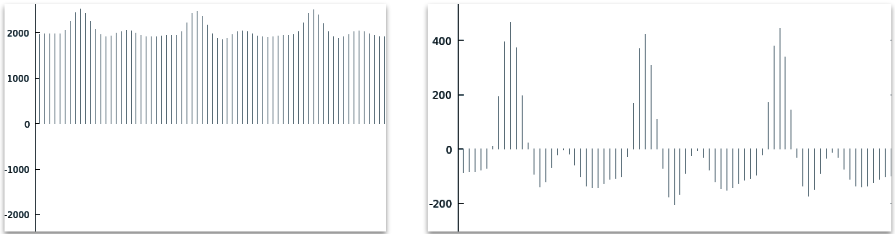
\includegraphics[width=0.9\textwidth]{AvancesPruebas/imagenes/offset.png}}
	\caption{Señal digital antes y después de aplicar el offset.}
	\label{fig:offset}
\end{figure}

Posteriormente se realiza el ventaneo de la señal digital aplicando la ventana de Hamming con un tamaño de $1600$ muestras. La ventana de Hamming está dada por la siguiente fórmula: 

\begin{equation}
\label{eq_hamming}
w(n) = 0.54 - 0.46 * cos(\frac{2\pi n}{N})
\end{equation}

Debido a que el cálculo de los $1600$ valores de la ventana, incrementa considerablemente el tiempo de procesamiento para cada muestra, se decidió almacenar los valores de la ventana en la memoria de programa del microcontrolador con el formato Q15, reduciendo así el tiempo de ejecución y evitando que se omitan valores dentro del tiempo de muestreo. \\

En la figura \ref{fig:ventaneo} se observa el resultado del ventaneo de la señal. \\

\begin{figure}[htbp!]
	\centering
	\fbox{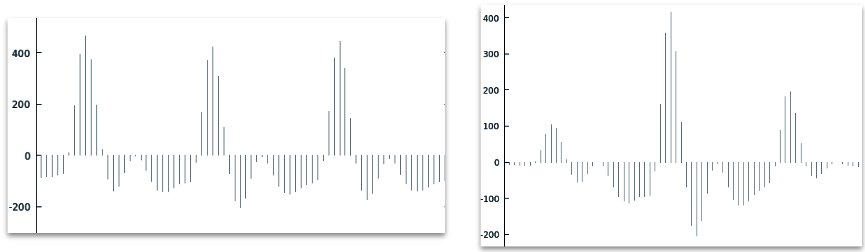
\includegraphics[width=0.9\textwidth]{AvancesPruebas/imagenes/ventaneo.png}}
	\caption{Señal digital antes y después de realizar el ventaneo.}
	\label{fig:ventaneo}
\end{figure}

Al término del cálculo de los valores de la autocorrelación, se realizó la búsqueda del segundo valor máximo (omitiendo el valor máximo ubicado en la posición $0$ del arreglo $Cxx$ ya que este corresponde con la energía de la señal, y la diferencia del máximo inicial al segundo máximo representa frecuencia fundamental de la señal) para obtener la posición de este valor y así poder calcular la frecuencia cardíaca con la fórmula (\ref{eq:lpm}). \\

En la figura \ref{fig:autocorr} se muestra el resultado de la autocorrelación y el valor máximo de interés del que se busca su posición. \\

\begin{figure}[htbp!]
	\centering
	\fbox{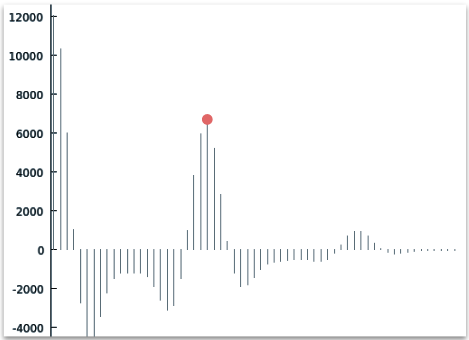
\includegraphics[width=0.6\textwidth]{AvancesPruebas/imagenes/autocorr.png}}
	\caption{Resultado de la autocorrelación de la señal digital de pulso cardíaco.}
	\label{fig:autocorr}
\end{figure}

\subsection{Pruebas unitarias}
En esta etapa se realizaron pruebas obteniendo la frecuencia cardíaca 10 veces a 8 personas de diferentes edades, y comparando el resultado obtenido con el esperado obtenido con el método de palpación se calculó el error porcentual de los resultados de las pruebas. En las tablas \ref{table:resultado1} y \ref{table:resultado2} se muestran los resultados obtenidos del cálculo de la frecuencia cardíaca comparado con el valor esperado. \\

\begin{table}[htbp]
	\centering
	\subfloat[Resultados Persona 1][Resultados de la Persona 1 con 23 años de edad y frecuencia cardíaca de \textbf{75 lpm}]{
		\begin{tabular}{|l|l|}
			\hline
			\textbf{lpm obtenidos} & \textbf{Error (\%)} \\
			\hline \hline
			75 & 0 \\
			\hline
			73 & 2.67 \\
			\hline
			76 & 1.33 \\
			\hline
			74 & 1.33 \\
			\hline
			73 & 2.67 \\
			\hline
			73 & 2.67 \\
			\hline
			73 & 2.67 \\
			\hline
			76 & 1.33 \\
			\hline
			76 & 1.33 \\
			\hline
			77 & 2.67 \\
			\hline
		\end{tabular}}
	\qquad
	\subfloat[Resultados Persona 2][Resultados de la Persona 2 con 54 años de edad y frecuencia cardíaca de \textbf{57 lpm}]{
		\begin{tabular}{|l|l|}
			\hline
			\textbf{lpm obtenidos} & \textbf{Error (\%)} \\
			\hline \hline
			57 & 0 \\
			\hline
			55 & 3.51 \\
			\hline
			56 & 1.75 \\
			\hline
			56 & 1.75 \\
			\hline
			57 & 0 \\
			\hline
			58 & 1.75 \\
			\hline
			56 & 1.75 \\
			\hline
			57 & 0 \\
			\hline
			57 & 0 \\
			\hline
			57 & 0 \\
			\hline
	\end{tabular}}

	\subfloat[Resultados Persona 3][Resultados de la Persona 3 con 17 años de edad y frecuencia cardíaca de \textbf{80 lpm}]{
		\begin{tabular}{|l|l|}
			\hline
			\textbf{lpm obtenidos} & \textbf{Error (\%)} \\
			\hline \hline
			79 & 1.25 \\
			\hline
			80 & 0 \\
			\hline
			80 & 0 \\
			\hline
			82 & 2.5 \\
			\hline
			80 & 0 \\
			\hline
			81 & 1.25 \\
			\hline
			80 & 0 \\
			\hline
			79 & 1.25 \\
			\hline
			81 & 1.25 \\
			\hline
			80 & 0 \\
			\hline
	\end{tabular}}
	\qquad
	\subfloat[Resultados Persona 4][Resultados de la Persona 4 con 64 años de edad y frecuencia cardíaca de \textbf{64 lpm}]{
		\begin{tabular}{|l|l|}
			\hline
			\textbf{lpm obtenidos} & \textbf{Error (\%)} \\
			\hline \hline
			65 & 1.56 \\
			\hline
			65 & 1.56 \\
			\hline
			64 & 0 \\
			\hline
			66 & 3.13 \\
			\hline
			64 & 0 \\
			\hline
			64 & 0 \\
			\hline
			64 & 0 \\
			\hline
			67 & 4.69 \\
			\hline
			65 & 1.56 \\
			\hline
			64 & 0 \\
			\hline
	\end{tabular}}

	\caption{Resultados del cálculo de la frecuencia cardíaca de las Personas 1 a 4.}
	\label{table:resultado1}
\end{table}

\begin{table}[htbp]
	\centering
	\subfloat[Resultados Persona 5][Resultados de la Persona 5 con 7 años de edad y frecuencia cardíaca de \textbf{86 lpm}]{
		\begin{tabular}{|l|l|}
			\hline
			\textbf{lpm obtenidos} & \textbf{Error (\%)} \\
			\hline \hline
			85 & 1.16 \\
			\hline
			86 & 0 \\
			\hline
			85 & 1.16 \\
			\hline
			84 & 2.33 \\
			\hline
			87 & 1.16 \\
			\hline
			86 & 0 \\
			\hline
			86 & 0 \\
			\hline
			87 & 1.16 \\
			\hline
			85 & 1.16 \\
			\hline
			85 & 1.16 \\
			\hline
	\end{tabular}}
	\qquad
	\subfloat[Resultados Persona 6][Resultados de la Persona 6 con 46 años de edad y frecuencia cardíaca de \textbf{73 lpm}]{
		\begin{tabular}{|l|l|}
			\hline
			\textbf{lpm obtenidos} & \textbf{Error (\%)} \\
			\hline \hline
			70 & 4.11 \\
			\hline
			72 & 1.37 \\
			\hline
			73 & 0 \\
			\hline
			73 & 0 \\
			\hline
			73 & 0 \\
			\hline
			72 & 1.37 \\
			\hline
			74 & 1.37 \\
			\hline
			75 & 2.74 \\
			\hline
			72 & 1.37 \\
			\hline
			72 & 1.37 \\
			\hline
	\end{tabular}}
	
	\subfloat[Resultados Persona 7][Resultados de la Persona 7 con 15 años de edad y frecuencia cardíaca de \textbf{68 lpm}]{
		\begin{tabular}{|l|l|}
			\hline
			\textbf{lpm obtenidos} & \textbf{Error (\%)} \\
			\hline \hline
			67 & 1.47 \\
			\hline
			67 & 1.47 \\
			\hline
			68 & 0 \\
			\hline
			69 & 1.47 \\
			\hline
			68 & 0 \\
			\hline
			68 & 0 \\
			\hline
			67 & 1.47 \\
			\hline
			69 & 1.47 \\
			\hline
			69 & 1.47 \\
			\hline
			66 & 2.94 \\
			\hline
	\end{tabular}}
	\qquad
	\subfloat[Resultados Persona 8][Resultados de la Persona 8 con 35 años de edad y frecuencia cardíaca de \textbf{82 lpm}]{
		\begin{tabular}{|l|l|}
			\hline
			\textbf{lpm obtenidos} & \textbf{Error (\%)} \\
			\hline \hline
			80 & 2.44 \\
			\hline
			81 & 1.22 \\
			\hline
			81 & 1.22 \\
			\hline
			82 & 0 \\
			\hline
			82 & 0 \\
			\hline
			82 & 0 \\
			\hline
			83 & 1.22 \\
			\hline
			81 & 1.22 \\
			\hline
			82 & 0 \\
			\hline
			84 & 2.44 \\
			\hline
	\end{tabular}}
	
	\caption{Resultados del cálculo de la frecuencia cardíaca de las Personas 5 a 8.}
	\label{table:resultado2}
\end{table}

En la tabla \ref{sensorPulso:promedioError} se muestra el promedio de los errores obtenidos en las pruebas realizadas a las 8 personas. \\

\begin{table}[htbp]
	\begin{center}
		\begin{tabular}{|l|l|l|}
			\hline
			\textbf{Edad (años)} & \textbf{Frecuencia cardíaca (lpm)} & \textbf{Error (\%)} \\
			\hline \hline
			23 & 75 & 1.87 \\
			\hline
			54 & 60 & 1.05 \\
			\hline
			17 & 80 & 0.75 \\
			\hline
			15 & 68 & 1.18\\
			\hline
			7 & 86 & 0.93 \\
			\hline
			64 & 63 & 1.25 \\
			\hline
			46 & 73 & 1.37 \\
			\hline
			35 & 82 & 0.98 \\
			\hline
		\end{tabular}
		\caption{Promedio de error de las pruebas del cálculo de frecuencia cardíaca.}
		\label{sensorPulso:promedioError}
	\end{center}
\end{table}

En la tabla \ref{sensorPulso:promedioError} se muestra el promedio de los errores obtenidos en las pruebas realizadas y se observa que se logró un error porcentual total de 1.17\%, que representa una diferencia de 1 o 2 latidos por minuto del resultado esperado.